\documentclass[trans]{beamer} 

\usepackage{selthcsslides}
\usepackage{tikz}
\usepackage{subfig}
\usepackage[toc,page]{appendix}
\usepackage{tikz}
\usepackage{pgfplots}
\usepackage{tikz}
\usepackage{pgfgantt}
\usepackage{xstring}
\usetikzlibrary{decorations.pathmorphing}
\usetikzlibrary{patterns}
\usetikzlibrary{arrows}
\usepackage{pgfplots}
\pgfplotsset{compat=1.10}
\usetikzlibrary{shapes.geometric,arrows,fit,matrix,positioning}
%\usecolortheme{lucolors}
\setbeamertemplate{navigation symbols}{}

% Swedish.
\usepackage[T1]{fontenc}
\usepackage[english]{babel}

\usepackage{url}

% Specifications.
\newlength{\specmargin}
\setlength{\specmargin}{\parindent}

\lstnewenvironment{Spec}
{\lstset{xrightmargin=\specmargin}
\lstset{print=true}
\lstset{frame=single}
\lstset{framesep=5pt}
\lstset{frameround=tttt}}
{}

\newcommand{\cinline}[1]{\lstinline[language=C]§#1§}

\lstnewenvironment{ccode}{
  \lstset{
    language=C,
    xleftmargin=4mm,
    tabsize=8,
    numberstyle=\small,
    stepnumber=1,
    numbersep=5pt,
    basicstyle=\ttfamily,
    identifierstyle=,
    commentstyle=\it,
    stringstyle=\ttfamily,
    showstringspaces=false
  }
}
{}

\newcommand{\specintro}[1]{\blankline {\small\hspace{1em} #1}\vspace{-1mm}}
\newcommand{\point}[1]{\centerline{\bf \em#1}}

\usetikzlibrary{decorations.pathmorphing}
\usetikzlibrary{patterns}
\usetikzlibrary{arrows}
\usepackage{pgfplots}
\pgfplotsset{compat=1.10}
\usetikzlibrary{shapes.geometric,arrows,fit,matrix,positioning}

\newcommand{\FIXAFTERCODE}{\vspace{-\baselineskip}}
\newcommand{\cancel}[1]{}
\input{alg}

\tikzset
{
    treenode/.style = {circle, draw=black, align=center, minimum size=8mm},
    subtree/.style  = {isosceles triangle, draw=black, align=center, minimum height=0.5cm, minimum width=1cm, shape border rotate=90, anchor=north}
}


%***************************************************************
\begin{document} 

\title{Lecture 2}
\author[jonasskeppstedt.net]{jonasskeppstedt.net}
\date{\input{year}} 

\newcommand{\vertexradius}[0]{7mm}
\newcommand{\vertexdistance}[0]{10mm}
\newcommand{\stddist}[0]{node distance = \vertexdistance}
\begin{frame}[fragile=singleslide]
\frametitle{Single linked list}
\begin{center}
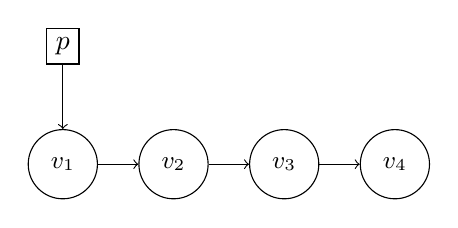
\begin{tikzpicture}[
      vertex/.style={circle, draw=black, inner sep=0pt, node distance=40pt,minimum size=25pt, font=\small}, pfeil/.style={->}]

\node[rectangle,draw=black] (v0) at (0,1.5) {$p$};
\node[vertex] (v1) at (0,0) {$v_1$};
\node[vertex,right of=v1] (v2) {$v_2$};
\node[vertex,right of=v2] (v3) {$v_3$};
\node[vertex,right of=v3] (v4) {$v_4$};
\draw[pfeil] (v0) edge (v1);
\draw[pfeil] (v1) edge (v2);
\draw[pfeil] (v2) edge (v3);
\draw[pfeil] (v3) edge (v4);

\end{tikzpicture}
\end{center}

\begin{ccode}
class List {
	int	data;
	List	next;
};

List	p;
\end{ccode}
\end{frame}

\begin{frame}[fragile=singleslide]
\frametitle{A corrupted single linked list}
\begin{center}
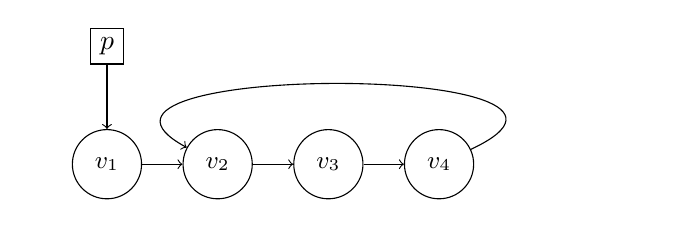
\begin{tikzpicture}[
      vertex/.style={circle, draw=black, inner sep=0pt, node distance=40pt,minimum size=25pt, font=\small}, pfeil/.style={->}]

\node[rectangle,draw=black] (v0) at (0,1.5) {$p$};
\node[vertex] (v1) at (0,0) {$v_1$};
\node[vertex,right of=v1] (v2) {$v_2$};
\node[vertex,right of=v2] (v3) {$v_3$};
\node[vertex,right of=v3] (v4) {$v_4$};
\draw[pfeil] (v0) edge (v1);
\draw[pfeil] (v1) edge (v2);
\draw[pfeil] (v2) edge (v3);
\draw[pfeil] (v3) edge (v4);
\draw[pfeil] (v4) .. controls (7,1.3) and (-1,1.3) .. (v2);

\end{tikzpicture}
\end{center}
\begin{itemize}
\item Quiz: how can you check if a list is corrupted without looping forever?
\end{itemize}
\end{frame}

\begin{frame}[fragile=singleslide]
\frametitle{Inserting a new node}
\begin{center}
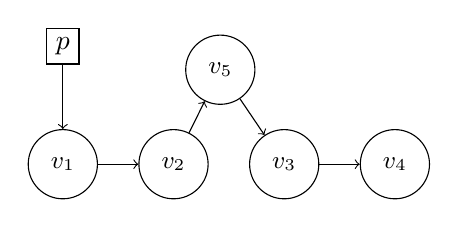
\begin{tikzpicture}[
      vertex/.style={circle, draw=black, inner sep=0pt, node distance=40pt,minimum size=25pt, font=\small}, pfeil/.style={->}]

\node[rectangle,draw=black] (v0) at (0,1.5) {$p$};
\node[vertex] (v1) at (0,0) {$v_1$};
\node[vertex,right of=v1] (v2) {$v_2$};
\node[vertex,right of=v2] (v3) {$v_3$};
\node[vertex,right of=v3] (v4) {$v_4$};
\node[vertex] (v5) at (2,1.2) {$v_5$};
\draw[pfeil] (v0) edge (v1);
\draw[pfeil] (v1) edge (v2);
\draw[pfeil] (v2) edge (v5);
\draw[pfeil] (v5) edge (v3);
\draw[pfeil] (v3) edge (v4);

\end{tikzpicture}
\end{center}
\begin{itemize}
\item Lists are more flexible than arrays
\end{itemize}
\end{frame}

\begin{frame}[fragile=singleslide]
\frametitle{Optimizing append}
\begin{center}
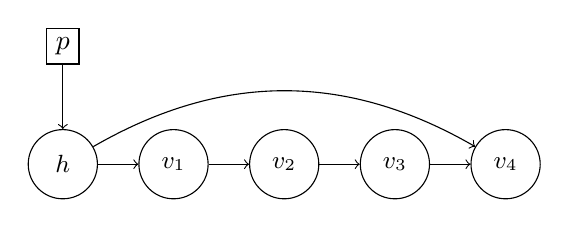
\begin{tikzpicture}[
      vertex/.style={circle, draw=black, inner sep=0pt, node distance=40pt,minimum size=25pt, font=\small}, pfeil/.style={->}]

\node[rectangle,draw=black] (v0) at (0,1.5) {$p$};
\node[vertex] (h) at (0,0) {$h$};
\node[vertex,right of=h] (v1) {$v_1$};
\node[vertex,right of=v1] (v2) {$v_2$};
\node[vertex,right of=v2] (v3) {$v_3$};
\node[vertex,right of=v3] (v4) {$v_4$};
\draw[pfeil] (v0) edge (h);
\draw[pfeil] (h) edge (v1);
\draw[pfeil] (h) edge[bend left] (v4);
\draw[pfeil] (v1) edge (v2);
\draw[pfeil] (v2) edge (v3);
\draw[pfeil] (v3) edge (v4);

\end{tikzpicture}
\end{center}
\begin{itemize}
\item A header node with pointers to both first and last nodes
\end{itemize}
\end{frame}

\begin{frame}[fragile=singleslide]
\frametitle{Double linked list}
\begin{center}
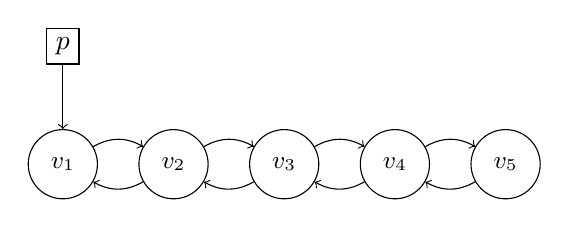
\begin{tikzpicture}[
      vertex/.style={circle, draw=black, inner sep=0pt, node distance=40pt,minimum size=25pt, font=\small}, pfeil/.style={->}]

\node[rectangle,draw=black] (v0) at (0,1.5) {$p$};
\node[vertex] (v1) at (0,0) {$v_1$};
\node[vertex,right of=v1] (v2) {$v_2$};
\node[vertex,right of=v2] (v3) {$v_3$};
\node[vertex,right of=v3] (v4) {$v_4$};
\node[vertex,right of=v4] (v5) {$v_5$};
\draw[pfeil] (v0) edge (v1);
\draw[pfeil] (v1) edge[bend left] (v2);
\draw[pfeil] (v2) edge[bend left] (v3);
\draw[pfeil] (v3) edge[bend left] (v4);
\draw[pfeil] (v4) edge[bend left] (v5);
\draw[pfeil] (v2) edge[bend left] (v1);
\draw[pfeil] (v3) edge[bend left] (v2);
\draw[pfeil] (v4) edge[bend left] (v3);
\draw[pfeil] (v5) edge[bend left] (v4);

\end{tikzpicture}
\end{center}
\begin{itemize}
\item More efficient in some situations
\end{itemize}
\end{frame}

\begin{frame}[fragile=singleslide]
\frametitle{A circular double linked list}
\begin{center}
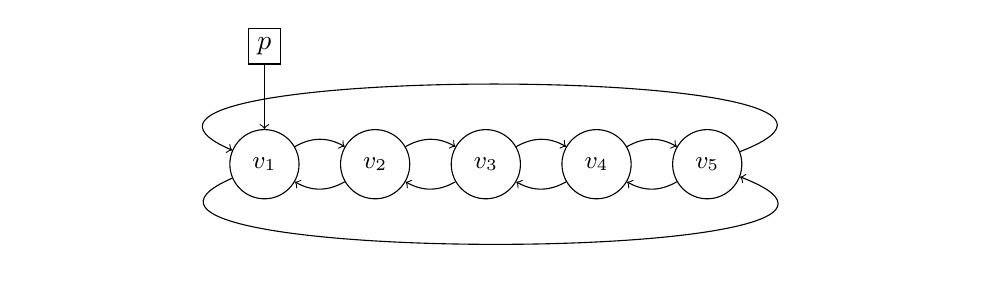
\begin{tikzpicture}[
      vertex/.style={circle, draw=black, inner sep=0pt, node distance=40pt,minimum size=25pt, font=\small}, pfeil/.style={->}]

\node[rectangle,draw=black] (v0) at (0,1.5) {$p$};
\node[vertex] (v1) at (0,0) {$v_1$};
\node[vertex,right of=v1] (v2) {$v_2$};
\node[vertex,right of=v2] (v3) {$v_3$};
\node[vertex,right of=v3] (v4) {$v_4$};
\node[vertex,right of=v4] (v5) {$v_5$};
\draw[pfeil] (v0) edge (v1);
\draw[pfeil] (v1) edge[bend left] (v2);
\draw[pfeil] (v2) edge[bend left] (v3);
\draw[pfeil] (v3) edge[bend left] (v4);
\draw[pfeil] (v4) edge[bend left] (v5);
\draw[pfeil] (v2) edge[bend left] (v1);
\draw[pfeil] (v3) edge[bend left] (v2);
\draw[pfeil] (v4) edge[bend left] (v3);
\draw[pfeil] (v5) edge[bend left] (v4);
\draw[pfeil] (v5) .. controls (9,1.3) and (-3,1.3) .. (v1);
\draw[pfeil] (v1) .. controls (-3,-1.3) and (9,-1.3) .. (v5);

\end{tikzpicture}
\end{center}
\begin{itemize}
\item Beware of infinite loops!
\item Often a do-while loop is convenient
\end{itemize}
\end{frame}

\begin{frame}[fragile=singleslide]
\frametitle{Binary search tree}
\begin{itemize}
\item A tree node $t$
\item {\em left(t)} $=$ {\em null} or {\em key(left(t))}$~<~${\em key(t)}
\item {\em right(t)} $=$ {\em null} or {\em key(right(t))}$~>~${\em key(t)}
\end{itemize}
\begin{itemize}
\item to {insert} a (key,value) pair,
\item to {delete} a node with a certain key, and
\item to {search} for a node with a certain key.
\end{itemize}
\end{frame}

\begin{frame}[fragile=singleslide]
\frametitle{Balanced binary search trees}
\begin{itemize}
\item Without balancing, the running time of insert, search, and delete would be $O(n)$ 
\item Two Russian mathematicians, Georgy Adelson-Velsky and Evgenii Landis, discovered in 1962 the first self-balancing binary search tree with $O(\log n)$ time for insert, delete, and search: the AVL-tree.
\item In 1972 the German computer scientist Rudolf Bayer invented another
self-balancing search tree: the red-black tree, with the same time complexity
\end{itemize}
\end{frame}

\begin{frame}[fragile=singleslide]
\frametitle{AVL tree balance attribute}
\begin{center}
\begin{tabular}{rl}
balance & meaning\\
\hline
$-1$ & left subtree is one higher than right subtree\\
$0$ & left and right subtrees have equal heights\\
$1$ & right subtree is one higher than left subtree\\
\hline
\end{tabular}
\end{center}

\end{frame}

\begin{frame}[fragile=singleslide]
\frametitle{Insertion}
\begin{center}
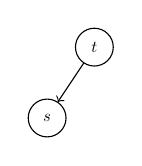
\begin{tikzpicture}[->,level/.style={sibling distance = 5cm/#1, level distance = 1.5cm},scale=0.6, transform shape]
\node [treenode] at (0,0) (s) {$s$};
\node [treenode] at (1.0,1.5) (t) {$t$};
\draw (t) edge (s);
\end{tikzpicture}
\begin{tikzpicture}
\node at (0,0) {};
\node at (0,1) {$\Rightarrow$};
\end{tikzpicture}
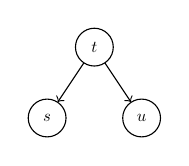
\begin{tikzpicture}[->,level/.style={sibling distance = 5cm/#1, level distance = 1.5cm},scale=0.6, transform shape]
\node [treenode] at (0,0) (s) {$s$};
\node [treenode] at (1.0,1.5) (t) {$t$};
\node [treenode] at (2,0) (u) {$u$};
\draw (t) edge (s);
\draw (t) edge (u);
\end{tikzpicture}

\end{center}

\end{frame}

\begin{frame}[fragile=singleslide]
\frametitle{Single rotations}
\begin{center}

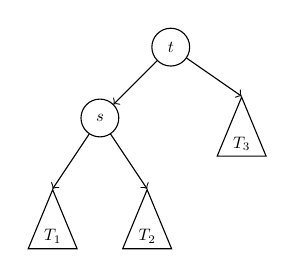
\begin{tikzpicture}[->,level/.style={sibling distance = 5cm/#1, level distance = 1.5cm},scale=0.6, transform shape]
\node [treenode] at (0,0) (s) {$s$};
\node [subtree] at (-1,-1.5) (t1) { $T_1$};
\node [subtree] at (1,-1.5) (t2) { $T_2$};
\node [treenode] at (1.5,1.5) (t) {$t$};
\node [subtree] at (3,0.46) (t3) { $T_3$};
\draw (s) edge (t1.north);
\draw (s) edge (t2.north);
\draw (t) edge (s);
\draw (t) edge (t3.north);
\end{tikzpicture}
\begin{tikzpicture}
\node at (0,0) {};
\node at (0,1) {$\Rightarrow$};
\end{tikzpicture}
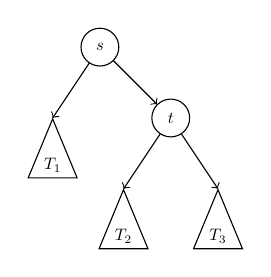
\begin{tikzpicture}[->,level/.style={sibling distance = 5cm/#1, level distance = 1.5cm},scale=0.6, transform shape]
\node [treenode] at (0,1.5) (s) {$s$};
\node [subtree] at (-1,0) (t1) { $T_1$};
\node [treenode] at (1.5,0) (t) {$t$};
\node [subtree] at (0.5,-1.5) (t2) { $T_2$};
\node [subtree] at (2.5,-1.5) (t3) { $T_3$};
\draw (s) edge (t1.north);
\draw (t) edge (t2.north);
\draw (s) edge (t);
\draw (t) edge (t3.north);
\end{tikzpicture}

\end{center}


\begin{center}

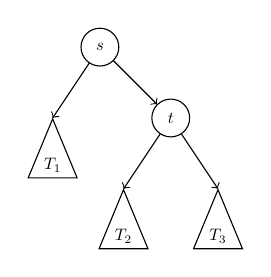
\begin{tikzpicture}[->,level/.style={sibling distance = 5cm/#1, level distance = 1.5cm},scale=0.6, transform shape]
\node [treenode] at (0,1.5) (s) {$s$};
\node [subtree] at (-1,0) (t1) { $T_1$};
\node [treenode] at (1.5,0) (t) {$t$};
\node [subtree] at (0.5,-1.5) (t2) { $T_2$};
\node [subtree] at (2.5,-1.5) (t3) { $T_3$};
\draw (s) edge (t1.north);
\draw (t) edge (t2.north);
\draw (s) edge (t);
\draw (t) edge (t3.north);
\end{tikzpicture}
\begin{tikzpicture}
\node at (0,0) {};
\node at (0,1) {$\Rightarrow$};
\end{tikzpicture}
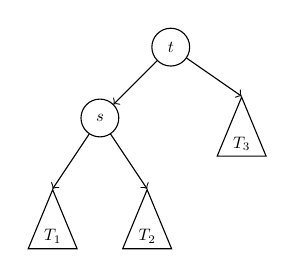
\begin{tikzpicture}[->,level/.style={sibling distance = 5cm/#1, level distance = 1.5cm},scale=0.6, transform shape]
\node [treenode] at (0,0) (s) {$s$};
\node [subtree] at (-1,-1.5) (t1) { $T_1$};
\node [subtree] at (1,-1.5) (t2) { $T_2$};
\node [treenode] at (1.5,1.5) (t) {$t$};
\node [subtree] at (3,0.46) (t3) { $T_3$};
\draw (s) edge (t1.north);
\draw (s) edge (t2.north);
\draw (t) edge (s);
\draw (t) edge (t3.north);
\end{tikzpicture}

\end{center}
\end{frame}

\begin{frame}[fragile=singleslide]
\frametitle{Double rotations}
\begin{center}

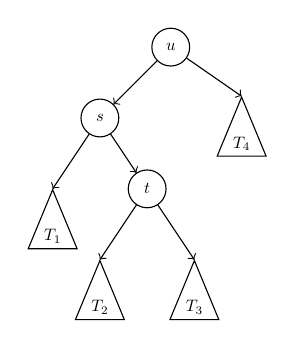
\begin{tikzpicture}[->,level/.style={sibling distance = 5cm/#1, level distance = 1.5cm},scale=0.6, transform shape]
\node [treenode] at (0,0) (s) {$s$};
\node [subtree] at (-1,-1.5) (t1) { $T_1$};
\node [treenode] at (1,-1.5) (t) { $t$};
\node [treenode] at (1.5,1.5) (u) {$u$};
\node [subtree] at (0.0,-3.0) (t2) { $T_2$};
\node [subtree] at (2.0,-3.0) (t3) { $T_3$};
\node [subtree] at (3.0,0.46) (t4) { $T_4$};
\draw (s) edge (t1.north);
\draw (t) edge (t2.north);
\draw (t) edge (t3.north);
\draw (s) edge (t);
\draw (u) edge (s);
\draw (u) edge (t4.north);
\end{tikzpicture}
\begin{tikzpicture}
\node at (0,0) {};
\node at (0,1.5) {$\Rightarrow$};
\end{tikzpicture}
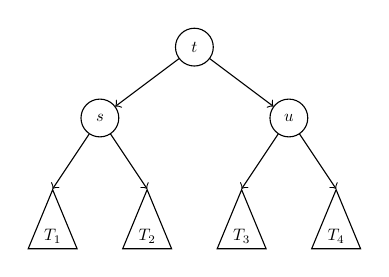
\begin{tikzpicture}[->,level/.style={sibling distance = 5cm/#1, level distance = 1.5cm},scale=0.6, transform shape]
\node [treenode] at (0,1.5) (t) {$t$};
\node [treenode] at (2.0,0) (u) {$u$};
\node [treenode] at (-2.0,0) (s) {$s$};
\node [subtree] at (-3.0,-1.5) (t1) { $T_1$};
\node [subtree] at (-1.0,-1.5) (t2) { $T_2$};
\node [subtree] at (1.0,-1.5) (t3) { $T_3$};
\node [subtree] at (3.0,-1.5) (t4) { $T_4$};
\draw (s) edge (t1.north);
\draw (s) edge (t2.north);
\draw (t) edge (s);
\draw (t) edge (u);
\draw (u) edge (t3.north);
\draw (u) edge (t4.north);
\end{tikzpicture}

\end{center}

\begin{center}

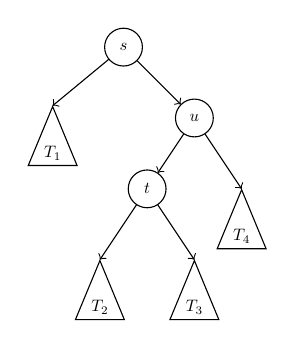
\begin{tikzpicture}[->,level/.style={sibling distance = 5cm/#1, level distance = 1.5cm},scale=0.6, transform shape]
\node [treenode] at (3,0) (u) {$u$};
\node [subtree] at (0.0,0.26) (t1) { $T_1$};
\node [treenode] at (2,-1.5) (t) { $t$};
\node [treenode] at (1.5,1.5) (s) {$s$};
\node [subtree] at (1.0,-3.0) (t2) { $T_2$};
\node [subtree] at (3.0,-3.0) (t3) { $T_3$};
\node [subtree] at (4.0,-1.5) (t4) { $T_4$};
\draw (s) edge (t1.north);
\draw (t) edge (t2.north);
\draw (t) edge (t3.north);
\draw (s) edge (u);
\draw (u) edge (t);
\draw (u) edge (t4.north);
\end{tikzpicture}
\begin{tikzpicture}
\node at (0,0) {};
\node at (0,1.5) {$\Rightarrow$};
\end{tikzpicture}
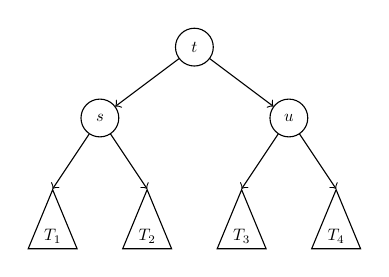
\begin{tikzpicture}[->,level/.style={sibling distance = 5cm/#1, level distance = 1.5cm},scale=0.6, transform shape]
\node [treenode] at (0,1.5) (t) {$t$};
\node [treenode] at (2.0,0) (u) {$u$};
\node [treenode] at (-2.0,0) (s) {$s$};
\node [subtree] at (-3.0,-1.5) (t1) { $T_1$};
\node [subtree] at (-1.0,-1.5) (t2) { $T_2$};
\node [subtree] at (1.0,-1.5) (t3) { $T_3$};
\node [subtree] at (3.0,-1.5) (t4) { $T_4$};
\draw (s) edge (t1.north);
\draw (s) edge (t2.north);
\draw (t) edge (s);
\draw (t) edge (u);
\draw (u) edge (t3.north);
\draw (u) edge (t4.north);
\end{tikzpicture}

\end{center}

\end{frame}


\begin{frame}[fragile=singleslide]
\frametitle{Hash maps or hash tables}
\begin{itemize}
\item Store (key,value) pairs using an array of size $m$
\item Insert, search and delete operations
\item Compute an index from the key (modulo $m$) using a hash function
\item When two keys are mapped to the same index there is a collision
\item Two main approaches to handle collisions:
\begin{itemize}
\item with separate chaining (\"oppen hashtabell)
\item with open addressing (sluten hashtabell)
\end{itemize}
\item With $n$ pairs, $\alpha = \frac{n}{m}$ is the load factor
\item Separate chaining uses linked lists for the pairs
\item Open addressing stores the pairs in the array
\end{itemize}
\end{frame}

\begin{frame}[fragile=singleslide]
\frametitle{Separate chaining}
\begin{itemize}
\item The table is an array of linked lists 
\item Compared with only one list, this will likely be $m$ times faster
\item Some alternatives:
\begin{itemize}
\item Always insert at the beginning (no search needed if you know it is a new pair)
\item Keep each list sorted 
\item Move frequently used pairs to the beginning of the list
\end{itemize}
\item Advantage: simple to implement
\item Disadvantage: less simple to allocate memory for the list nodes efficiently (allocation and freeing/garbage collecting nodes takes time)
\item Usually a good choice
\item If $\alpha$ gets too big, the operations will be slower but still work
\item Resize array if needed
\end{itemize}
\end{frame}

\begin{frame}[fragile=singleslide]
\frametitle{Open addressing}
\begin{itemize}
\item Invented by Gene Amdahl (known for Amdahl's law)
\item $\alpha < 1$ (but see below --- significantly less than one is better)
\item Three ways to handle collisions
\begin{itemize}
\item Linear probing
\item Quadratic probing
\item Double hashing probing
\end{itemize}
\end{itemize}
\end{frame}

\begin{frame}[fragile=singleslide]
\frametitle{Linear probing}
\begin{itemize}
\item An array element either contains a pair or a value ''empty'' (e.g. null)
\item Sometimes it is simpler to have one array for keys and another for values, with the key and value of a pair 
stored at index $i$ in the two arrays
\item First compute an index $i \leftarrow f(key) \mod m$
\item If $a[i]$ is not empty, set $i \leftarrow (i + 1)\mod m$ and check again
\item Otherwise insert new pair at $i$
\item Similar for search
\item Quiz: can we do the same for delete plus storing ''empty'' in the array?
\end{itemize}
\end{frame}

\begin{frame}[fragile=singleslide]
\frametitle{Linear probing: delete}
\begin{itemize}
\item Answer: no, since we then might not find some of the keys.
\item Empty hash table:
\begin{tabular}{|p{1cm}|p{1cm}|p{1cm}|p{1cm}|p{1cm}|p{1cm}|p{1cm}|}
\hline 
empty & empty & empty & empty & empty & empty & empty \\
\hline 
\end{tabular}

\item Insert two pairs with $f(k_1) \mod m = f(k_2) \mod m$
\begin{tabular}{|p{1cm}|p{1cm}|p{1cm}|p{1cm}|p{1cm}|p{1cm}|p{1cm}|}
\hline 
empty & $k_1$ & $k_2$ & empty & empty & empty & empty \\
\hline 
\end{tabular}
\item Delete the pair $k_1$
\begin{tabular}{|p{1cm}|p{1cm}|p{1cm}|p{1cm}|p{1cm}|p{1cm}|p{1cm}|}
\hline 
empty & empty & $k_2$ & empty & empty & empty & empty \\
\hline 
\end{tabular}
\item Search for $k_2$
\begin{tabular}{|p{1cm}|p{1cm}|p{1cm}|p{1cm}|p{1cm}|p{1cm}|p{1cm}|}
\hline 
empty & empty & $k_2$ & empty & empty & empty & empty \\
\hline 
\end{tabular}

will give up at first probe since it sees ''empty''
\item What can we do? Quiz: why not store a value ''deleted'' and skip such when searching?
\end{itemize}
\end{frame}


\begin{frame}[fragile=singleslide]
\frametitle{Linear probing: delete}
\begin{itemize}
\item Answer: yes, that works but gives other problems
\item Empty hash table:
\begin{tabular}{|p{1cm}|p{1cm}|p{1cm}|p{1cm}|p{1cm}|p{1cm}|p{1cm}|}
\hline 
empty & empty & empty & empty & empty & empty & empty \\
\hline 
\end{tabular}

\item Insert two pairs with $f(k_1) \mod m = f(k_2) \mod m$
\begin{tabular}{|p{1cm}|p{1cm}|p{1cm}|p{1cm}|p{1cm}|p{1cm}|p{1cm}|}
\hline 
empty & $k_1$ & $k_2$ & empty & empty & empty & empty \\
\hline 
\end{tabular}
\item Delete the pair $k_1$
\begin{tabular}{|p{1cm}|p{1cm}|p{1cm}|p{1cm}|p{1cm}|p{1cm}|p{1cm}|}
\hline 
empty & deleted & $k_2$ & empty & empty & empty & empty \\
\hline 
\end{tabular}
\item Search for $k_2$
\begin{tabular}{|p{1cm}|p{1cm}|p{1cm}|p{1cm}|p{1cm}|p{1cm}|p{1cm}|}
\hline 
empty & deleted & $k_2$ & empty & empty & empty & empty \\
\hline 
\end{tabular}

will skip ''deleted'' and find $k_2$
\item Quiz: when is this bad?
\end{itemize}
\end{frame}

\begin{frame}[fragile=singleslide]
\frametitle{Storing ''deleted''}
\begin{itemize}
\item Answer: we may store many ''deleted'' that must be skipped
\item But if we insert and come to a ''deleted'' then we can use that position.
\item I use the words position and index for the same place in the array but it is a slight abuse of English.
\item If we have too many ''deleted'' we can clean the hash table to remove them by reinserting everything
\item Quiz: instead of storing ''deleted'', can we not move items ''to the left''?
\end{itemize}
\end{frame}


\begin{frame}[fragile=singleslide]
\frametitle{Linear probing: delete with move}
\begin{itemize}
\item Answer: yes, if we are careful
\item Empty hash table:
\begin{tabular}{|p{1cm}|p{1cm}|p{1cm}|p{1cm}|p{1cm}|p{1cm}|p{1cm}|}
\hline 
empty & empty & empty & empty & empty & empty & empty \\
\hline 
\end{tabular}

\item Insert two pairs with $f(k_1) \mod m = f(k_2) \mod m$
\begin{tabular}{|p{1cm}|p{1cm}|p{1cm}|p{1cm}|p{1cm}|p{1cm}|p{1cm}|}
\hline 
empty & $k_1$ & $k_2$ & empty & empty & empty & empty \\
\hline 
\end{tabular}
\item Delete the pair $k_1$ and move $k_2$
\begin{tabular}{|p{1cm}|p{1cm}|p{1cm}|p{1cm}|p{1cm}|p{1cm}|p{1cm}|}
\hline 
empty & $k_2$ & empty & empty & empty & empty & empty \\
\hline 
\end{tabular}
\item Search for $k_2$
\begin{tabular}{|p{1cm}|p{1cm}|p{1cm}|p{1cm}|p{1cm}|p{1cm}|p{1cm}|}
\hline 
empty & $k_2$ & empty & empty & empty & empty & empty \\
\hline 
\end{tabular}

will find $k_2$
\item Quiz: what could go wrong?
\end{itemize}
\end{frame}


\begin{frame}[fragile=singleslide]
\frametitle{Linear probing: delete with bad move}
\begin{itemize}
\item Answer: moving a key to the left of its originally computed index
\item Insert two pairs with $f(k_1) \mod m = f(k_2) \mod m$
\begin{tabular}{|p{1cm}|p{1cm}|p{1cm}|p{1cm}|p{1cm}|p{1cm}|p{1cm}|}
\hline 
empty & $k_1$ & $k_2$ & empty & empty & empty & empty \\
\hline 
\end{tabular}

\item Insert a pair with $f(k_0) \mod m = 0$
\begin{tabular}{|p{1cm}|p{1cm}|p{1cm}|p{1cm}|p{1cm}|p{1cm}|p{1cm}|}
\hline 
$k_0$ & $k_1$ & $k_2$ & empty & empty & empty & empty \\
\hline 
\end{tabular}

\item Delete $k_1$ and move $k_2$
\begin{tabular}{|p{1cm}|p{1cm}|p{1cm}|p{1cm}|p{1cm}|p{1cm}|p{1cm}|}
\hline 
$k_0$ & $k_2$ & empty & empty & empty & empty & empty \\
\hline 
\end{tabular}
\item Delete $k_0$ and move $k_2$
\begin{tabular}{|p{1cm}|p{1cm}|p{1cm}|p{1cm}|p{1cm}|p{1cm}|p{1cm}|}
\hline 
$k_2$ & empty & empty & empty & empty & empty & empty \\
\hline 
\end{tabular}

will never find $k_2$
\end{itemize}
\end{frame}

\begin{frame}[fragile=singleslide]
\frametitle{Linear probing: correct delete with move}
{\small
\begin{tabbing}
\ahdr
\PROC \CALL{delete}($k$, $h$)				\\
\BEGIN							\\
\>$i\leftarrow h(k) \mod m$ 				\\
\>\WHILE true \DO \{					\\
\>\>$a[i]\leftarrow$ {\em empty}				\\
\>\>$j\leftarrow i$ 					\\
\>\>\WHILE true \DO \{					\\
\>\>\>$i\leftarrow (i+1)\mod m$				\\
\>\>\>\IF $a[i] = $ {\em empty} \THEN				\\
\>\>\>\>\RETURN						\\
\>\>\>$k\leftarrow h(a[i]) \mod m$ 			\\
\>\>\>\IF \NOT ($j \le k < i$ \OR $i \le j < k$ \OR $k < i < j$) \THEN				\\
\>\>\>\>$a[j]\leftarrow$ a[i]				\\
\>\>\>\>\BREAK									\\
\>\}							\\
\END
\end{tabbing}
}
\begin{itemize}
\item Three conditions needed due to modulo m.
\end{itemize}
\end{frame}

\begin{frame}[fragile=singleslide]
\frametitle{A simple model of unsuccessful search in linear probing}
\begin{itemize}
\item We ignore clustering and instead assume all positions are equally likely to be occupied. 
\item If the random variable $X$ is the number of probes in an unsuccessful search, what is 
 the expected value of $X$, $\mathbb{E}[X]$?
\item $\probP(X \ge k)$ is the probability that the first $k-1$ positions are occupied, and the last is empty. 
\begin{itemize}
\item The probability the first probed is occupied is: $\frac{n}{m}$,
\item the two first: $\frac{n}{m} \cdot \frac{n-1}{m-1}$,
\end{itemize}
\item

\item For $k > 1$ we can write:
\[
\begin{array}{ccc}
\probP(X \ge k) &=& \frac{n}{m} \cdot \frac{n-1}{m-1} \cdot ... \cdot \frac{n-k+2}{m-k+2} \le (\frac{n}{m})^{k-1} = \alpha^{k-1},
\end{array}
\]
\item with the last expression is valid also for $k=1$.
\end{itemize}
\end{frame}

\begin{frame}[fragile=singleslide]
\frametitle{A simple formula for $\mathbb{E}[X]$}

{\small
\[
\begin{array}{ccc}
\mathbb{E}[X] &=&\sum\limits_{k=1}^{\infty} k\cdot\probP(X = k)			\\
 &=&\sum\limits_{k=1}^{\infty} k\cdot(\probP(X \ge k)-\probP(X \ge k+1))	\\
 &=&1\cdot \probP(X \ge 1)-1\cdot \probP(X \ge 2)\\
 &&+~2\cdot \probP(X \ge 2)-2\cdot \probP(X \ge 3)\\
 &&+~3\cdot \probP(X \ge 3)-3\cdot \probP(X \ge 4)\\
 && ...\\
 &=&1\cdot \probP(X \ge 1)\\
 &&+~2\cdot \probP(X \ge 2)\\
 &&+~3\cdot \probP(X \ge 3)\\
 && ...\\
 &=&\sum\limits_{k=1}^{\infty} \probP(X \ge k)					\\
 &\le&\sum\limits_{k=1}^{\infty} \alpha^{k-1}					\\
 &=&\sum\limits_{k=0}^{\infty} \alpha^{k}= \frac{1}{1-\alpha},~\mathrm{since}~\alpha < 1.
\end{array}
\]
}

\end{frame}
\begin{frame}[fragile=singleslide]
\frametitle{Max expected number of probes in an unsuccessful search}

\begin{table}[H]
\begin{center}
\begin{tabular}{|c|c|}
\hline
$\alpha$ & $\mathbb{E}[X]$\\
\hline
0.2 & 1.25\\
0.3 & 1.43\\
0.4 & 1.67\\
0.5 & 2.00\\
0.6 & 2.50\\
0.7 & 3.33\\
0.8 & 5.00\\
0.9 & 10.00\\
0.95 & 20.00\\
0.98 & 50.00\\
\hline
\end{tabular}
\end{center}
\end{table}
\begin{itemize}
\item Recall this is an optimistic estimation since clustering is ignored
\item In reality, long sequences of occupied positions tend to grow longer
\item See Knuth TAOCP Volume 3 for a more detailed analysis
\item This analysis is sufficient to convince us to avoid large $\alpha$
\end{itemize}
\end{frame}



\begin{frame}[fragile=singleslide]
\frametitle{Quadratic probing}
\begin{itemize}

\item
The purpose of quadratic probing is to reduce the risk of clustering by adding $i^2$ instead of only $i$
to the initial hash value. 
\item The intent is to leave a cluster quickly. 
\item Below $h^\prime$ is the original hash function 

\[
\begin{array}{ccc}
h(k, i) &=& (h^\prime(k) + i^2) \mod m
\end{array}
\]

\item Clustering is reduced but if two different keys have the same hash value, there can be 
{secondary clustering} since
the positions probed for these keys will be the same. 
\item Quiz: can we now know we will find an empty position if there is one?
\end{itemize}
\end{frame}
\begin{frame}[fragile=singleslide]
\frametitle{Quadratic probing}
\begin{itemize}

\item Answer: no
\item Assume $m = 3$ and $h^\prime(k) = 0$ 
\item This is a very bad ''hash function'' but for illustration only, but during debugging it can be useful
\item The sequence of visited positions would initally be: $(0, 1, 1)$ from\\
$(0, (0+1^2)\mod 3 = 1, (0+2^2)\mod 3 = 1)$
\item We number the probings as probe $0, 1, 2$
\item We miss position $2$ since different probe numbers are mapped to the same position
\item Note it did not help that $m$ is a prime number --- at least not for now
\item Quiz: can we add a constraint to make this work?
\end{itemize}
\end{frame}

\begin{frame}[fragile=singleslide]
\frametitle{Making quadratic probing work better}
\begin{itemize}
\item Answer: yes. 
\item If $m$ is prime and we also require that $\alpha = n/m < \frac{1}{2}$, it will work.
\item Let $i$ and $j$ be the probe numbers made for two different searches or insertions.
\item Assume both operations resulted in the same hash value so they start searching at the same
positions.
\item $i$ and $j$ will start at one, be incremented, and probe until an empty position is found.
\item Assume the operation using $i$ inserted something first, somewhere.
\item The operation using $j$ will initially use the same positions, i.e. same values as $i$.
\item We want to show that when $i$ and $j$ have {\em different values} they would not map to the same positions
\item That means $j$ does not ''return to'' a position in the sequence used by $i$.
\end{itemize}
\end{frame}

\begin{frame}[fragile=singleslide]
\frametitle{A lemma}
\begin{lemma}
If $m$ is prime and $\alpha = \frac{n}{m} < \frac{1}{2}$, and $i\ne j$, then quadratic probing will find an empty position in
less than $\frac{m}{2}$ probes
\end{lemma}
\end{frame}


\begin{frame}[fragile=singleslide]
\frametitle{A proof}
\begin{proof}
{Let $0\le i, j < \lceil \frac{m}{2}\rceil$, and $h^\prime(k_1) = h^\prime(k_2)$. Assume incorrectly that two different probe numbers, $i$ and $j$, are mapped to the same positions.}
\[
\begin{array}{ccc}
(h^\prime(k_1) + i^2) \mod m &=& (h^\prime(k_2) + j^2) \mod m\\
(h^\prime(k_1) + i^2) &\equiv& (h^\prime(k_2) + j^2) \mod m\\
i^2 &\equiv& j^2 \mod m\\
i^2 - j^2 &\equiv& 0 \mod m\\
(i-j)(i+j) &\equiv& 0 \mod m\\
\end{array}
\]

Since $m$ is prime and $i\neq j$, either $i-j$ or $i+j$ is divisible by $m$, but since both $i-j$ and $i+j$ are less than $m$,
none of them can be divisible by $m$. A contradiction.
Therefore the first $\lceil \frac{m}{2}\rceil$ probes are to different positions and since $\alpha < \frac{1}{2}$,
an empty position will be found.
\end{proof}
\end{frame}

\begin{frame}[fragile=singleslide]
\frametitle{Double hashing}
\begin{itemize}

\item
Another alternative is to use an additional hash function:
\[
\begin{array}{ccc}
h(k, i) &=& (h_1(k) + i\cdot h_2(k)) \mod m
\end{array}
\]
\item
Assume two different keys had the same hash value in quadratic probing, i.e., with $h_1(k)$.
\item Then it is hoped that the risk that they have the same value also for $h_2(k)$ is much less.
\item In practice this removes most clustering.
\item
By guaranteeing that $h_2(k)$ is relatively prime to $m$, all positions will be probed. Two simple ways
to achieve this are:
\begin{itemize}
\item let $m = 2^n$ and ensure that $h_2(k)$ always is odd, or
\item let $m$ be prime and $0 < h_2(k) < m$.
\end{itemize}
\end{itemize}
\end{frame}

\begin{frame}[fragile=singleslide]
\frametitle{Summary of hash tables}
\begin{itemize}
\item No obvious ''best'' choice
\item Luckily both alternatives are easy to implement.
\item Best is to make performance measurements before changing anything, obviously. 
\item Especially the number of cache misses can explain performance differences.
\item See EDAG01 for profilers for C (and C++).
\item In EDAG01 you will even use a simulator from IBM which explains what happens each clock cycle in a modern CPU (POWER8).
\end{itemize}
\end{frame}
\cancel{

\subsection{\label{data.hash.summary.sec}Summary of hash tables}

Which hash table to use depends on the context but a clear advantage with
open addressing is much better locality of references which can lead to significantly better cache performance~\cite{cbook}.
Although it may appear to be simpler to use separate chaining, it can be more complicated to make efficient use of memory when
allocating and deallocating (or garbage collecting) the list nodes in separate chaining.
Assuming the cost of computing $h_2$ in double hashing is sufficiently low (which may be false), open 
addressing with double hashing
appears to be the most preferable hash table in a performance critical application, it is of course 
necessary to make performance measurements~\cite{cbook}. On the other hand, it is simpler to use separate chaining
and the performance may be sufficient.
}

\begin{frame}[fragile=singleslide]
\frametitle{Graphs}
\begin{itemize}
\item Notation
\item Graph traversal and connectivity
\item Testing bipartiteness
\item Connectivity in directed graphs
\end{itemize}
\end{frame}



\begin{frame}[fragile=singleslide]
\frametitle{Graphs}


\begin{columns}
\begin{column}{5cm}
{\small \tt
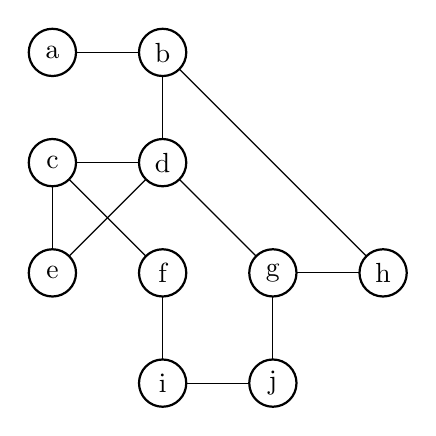
\begin{tikzpicture}
\tikzstyle{vertex}=[circle, inner sep=1pt,outer sep=0pt, 
	thick, node distance = 14mm,draw=black,minimum height=6mm,
]
\node[vertex] (a) { a };
\node[right of = a,vertex] (b) { b };
\node[below of = a,vertex] (c) { c };
\node[right of = c,vertex] (d) { d };
\node[below of = c,vertex] (e) { e };
\node[right of = e,vertex] (f) { f };
\node[right of = f,vertex] (g) { g };
\node[right of = g,vertex] (h) { h };
\node[below of = f,vertex] (i) { i };
\node[below of = g,vertex] (j) { j };
\path[-] (a) edge (b) ;
\path[-] (e) edge (c) ;
\path[-] (e) edge (d) ;
\path[-] (d) edge (c) ;
\path[-] (f) edge (c) ;
\path[-] (f) edge (i) ;
\path[-] (g) edge (h) ;
\path[-] (g) edge (j) ;
\path[-] (b) edge (d) ;
\path[-] (d) edge (g) ;
\path[-] (i) edge (j) ;
\path[-] (b) edge (h) ;

\end{tikzpicture}
}
\end{column}

\begin{column}{6cm}
\begin{itemize}
\item $G = (V,E)$
\item $V$ is a set of nodes or vertices
\item $E$ is a set of edges or arcs
\item $V = \{ a,b,c,d,e,f,g,h,i,j \}$
\item $E = \{ a-b,b-d, ..., i-j \}$, or
\item $E = \{ (a,b), (b,d), ..., (i,j) \}$
\item $n = |V|$
\item $m = |E|$
\end{itemize}
\end{column}
\end{columns}
\end{frame}

\begin{frame}
\frametitle{Example graphs}
\begin{itemize}
\item Cities connected by direct air flights: node = city, edge = flight
\item Social networks: node = person, edge = friend
\item An {\bf undirected graph} describes friends on a social network
\item When you follow somebody you have an edge from one to another, i.e. a {\bf directed graph}
\item Actually, we can view city connectivity through air flights as a directed graph but normally there is a flight back
\item Chess games: node = position, edge = legal move
\end{itemize}
\end{frame}

\begin{frame}
\frametitle{Graph representation: adjacency matrix}
\begin{itemize}
\item $n = |V|$ and $m = |E|$
\item Number each vertex from $1..n$
\item Often two representations of each edge
\item If there is an edge $i-j$ then
one is stored both in $m[i][j]$ and in $m[j][i]$, otherwise a zero 
\item If $n$ is large it can be a good idea to store only half the matrix
\item $\Theta(n^2)$ space
\item $\Theta(1)$ time to check if there is an edge $i-j$
\item $\Theta(n)$ time to find all neighbors of a node
\item $\Theta(n^2)$ time to list all edges
\end{itemize}
\end{frame}

\begin{frame}
\frametitle{Graph representation: adjacency list}
\begin{itemize}
\item $n = |V|$ and $m = |E|$
\item Every vertex has a list of neighbors
\item Every edge $u-v$ is stored in both $u$ and $v$
\item $degree(n)$ is the number of neighbors
\item $\Theta(degree(n))$ time to find all neighbors of a node
\item $\Theta(m)$ time to list all edges
\end{itemize}
\end{frame}

\begin{frame}
\frametitle{Optimizations}
\begin{itemize}
\item Store only half of the adjacency matrix for undirected graphs
\item For a very dense graph the matrix is smaller and just as fast
\item If you need both quick neighbor check and being able to quickly list all neighbors, then use both!
\item Optimizing compilers use both when deciding which variable should be allocated a processor register:
the variables are nodes and there is an edge $x-y$ if $x$ and $y$ may be needed at the same time (and therefore cannot use the same register)
\end{itemize}
\end{frame}

\begin{frame}
\frametitle{Paths and connectivity}
\begin{itemize}
\item A {\bf path}  is a sequence of nodes $p = (v_1, v_2, ... , v_k)$ such that $v_i$ and $v_{i+1}$ are neighbors in 
an undirected graph, or there is an edge from $v_i$ to $v_{i+1}$ in a directed graph.
\item If all nodes in $p$ are distinct then it is a {\bf simple path}.
\item An undirected graph is {\bf connected} if there is a path between every pair of nodes.
\item A {\bf cycle} is a path which consists of a simple path followed by the first node such as $(u,v,w,u)$.
\end{itemize}
\end{frame}

\begin{frame}
\frametitle{Trees}
\begin{itemize}
\item A connected undirected graph is a {\bf tree} if it has no cycle.
\item A tree has $n-1$ edges.
\item In a {\bf rooted tree} one node, $r$ is called the node.
\end{itemize}
\end{frame}

\begin{frame}[fragile=singleslide]
\frametitle{Depth first search: DFS}
{\small
\begin{tabbing}
\ahdr
\INT \>\ID{dfnum};\>\>\>\>\>/* Depth-first search number. */	\\
\PROC \CALL{dfs}($v$)						\\
\BEGIN								\\
\>\CALL{dfn}($v$) \ASGN \ID{dfnum}				\\
\>\CALL{visited}($v$) \ASGN true				\\
\>\ID{dfnum} \ASGN \ID{dfnum} $ + 1$				\\
								\\
\>\FOR each $w \in succ(v)$ \DO					\\
\>\>\IF (\NOT \CALL{visited}($w$)) 				\\
\>\>\>\CALL{dfs}($w$)						\\
\END
\ahdr
\PROC \NC{depth\_first\_search}{V}				\\
\>\ID{dfnum} \ASGN $0$						\\
\>\FOR each $v \in V$ \DO					\\
\>\>\CALL{visited}($v$) \ASGN false				\\
\>\CALL{dfs}($s$)				\\
\END
\end{tabbing}
}
\end{frame}

\begin{frame}
\frametitle{DFS}
\begin{itemize}
\item Properties of depth-first search have been studied extensively by Robert Tarjan
\item DFS is used a lot in compilers
\item His algorithms tend to be faster than others' and often more beautiful than art
\end{itemize}
\end{frame}

\begin{frame}[fragile=singleslide]
\frametitle{DFS example}
\begin{center}
{\tiny
\begin{tikzpicture}[thick]

\tikzstyle{vertex1}=[circle,thick, draw=black,
inner sep=0pt,outer sep=40pt,minimum size=\vertexradius]
\tikzstyle{vertex}=[circle,thick, node distance = 1.8*\vertexdistance,draw=black,minimum height=\vertexradius]
\node[vertex] at (0,0)	(0) {$0$}; 
\node[vertex,below of = 0, node distance = \vertexdistance] (1) {$1$};
\draw[->] (0) edge (1) ;
\node[vertex,below of =1,xshift=-\vertexdistance ](2) {$2$} ;
\draw[->] (1) edge (2) ;
\node[vertex,below of =1,xshift=\vertexdistance ](5) {$5$} ;
\draw[->] (1) edge (5) ;
\node[vertex,below of =2,xshift=\vertexdistance ](3) {$3$} ;
\draw[->] (2) edge (3) ;
\draw[->] (1) edge (3) ;
\draw[->] (5) edge (3) ;
\node[vertex,below of =3](4) {$4$} ;
\node[vertex,below of =5](6) {$6$} ;
\draw[->] (3) edge (4) ;
\draw[->] (5) edge (6) ;
\draw[->] (6) edge (4) ;
\draw[->] (3) .. controls (-3,-9) and (-3,1) .. (1);
\end{tikzpicture}
}
{\tiny
\begin{tikzpicture}[thick]

\tikzstyle{vertex1}=[circle,thick, draw=black,
inner sep=0pt,outer sep=40pt,minimum size=\vertexradius]
\tikzstyle{vertex}=[circle,thick, node distance = 1.8*\vertexdistance,draw=black,minimum height=\vertexradius]
\node[vertex] at (0,0)	(0) {$0$}; 
\node[vertex,below of = 0, node distance = \vertexdistance] (1) {$1$};
\draw[solid,->] (0) edge node[right] {\em tree} (1) ;
\node[vertex,below of =1,xshift=-\vertexdistance ](2) {$2$} ;
\draw[solid,->] (1) edge node[left] {\em tree\ \ } (2) ;
\node[vertex,below of =1,xshift=\vertexdistance ](5) {$5$} ;
\draw[->] (1) edge node[right] {\em tree} (5) ;
\node[vertex,below of =2,xshift=\vertexdistance ](3) {$3$} ;
\draw[solid,->] (2) edge node[left] {\em tree\ \ } (3) ;
\draw[dotted,->] (1) edge node [sloped,below] {\em forward} (3);
\draw[loosely dotted,->] (5) edge node [sloped,above] {\em cross} (3) ;
\node[vertex,below of =3](4) {$4$} ;
\node[vertex,below of =5](6) {$6$} ;
\draw[solid,->] (3) edge node[left] {\em tree} (4) ;
\draw[solid,->] (5) edge node[right] {\em tree} (6) ;
\draw[loosely dotted,->] (6) edge node [right] {\em cross} (4) ;
\draw[dashed,->] (3) .. controls (-3,-9) and (-3,1) .. node[near end,left]{\em cycle\ \ } (1);
\end{tikzpicture}
}
\end{center}
\end{frame}
\begin{frame}
\frametitle{The s-t connectivity problem}
\begin{itemize}
\item The problem is to find a path from $s$ to $t$.
\item Often we want to find the shortest path from $s$ to $t$.
\item The {\bf distance} between two nodes $u$ and $v$ is the number of
edges on a shortest path from $u$ to $v$
\item How to solve the connectivity problem? 
\item Check all nodes $v$ at a distance $k$ from $s$ until
either $v = t$ or there are no more nodes to check, in which case $s$ and $t$ are not
connected.
\item Let $k = 1, 2, 3, ..., \infty$
\item This is called {\bf breadth first search}, or simply {\bf BFS}
\item Think of an onion. You start in the center and explore one layer at a time outwards. 
\end{itemize}
\end{frame}

\begin{frame}
\frametitle{Breadth first search}
\begin{columns}
\begin{column}{5cm}
{\small \tt
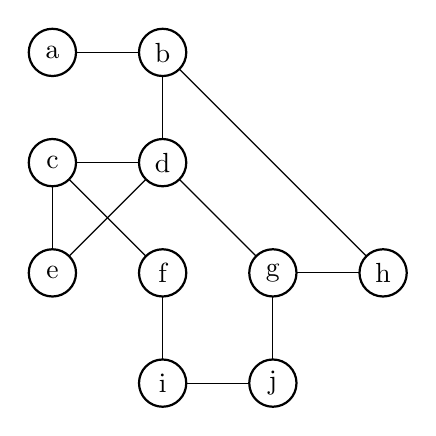
\begin{tikzpicture}
\tikzstyle{vertex}=[circle, inner sep=1pt,outer sep=0pt, 
	thick, node distance = 14mm,draw=black,minimum height=6mm,
]
\node[vertex] (a) { a };
\node[right of = a,vertex] (b) { b };
\node[below of = a,vertex] (c) { c };
\node[right of = c,vertex] (d) { d };
\node[below of = c,vertex] (e) { e };
\node[right of = e,vertex] (f) { f };
\node[right of = f,vertex] (g) { g };
\node[right of = g,vertex] (h) { h };
\node[below of = f,vertex] (i) { i };
\node[below of = g,vertex] (j) { j };
\path[-] (a) edge (b) ;
\path[-] (e) edge (c) ;
\path[-] (e) edge (d) ;
\path[-] (d) edge (c) ;
\path[-] (f) edge (c) ;
\path[-] (f) edge (i) ;
\path[-] (g) edge (h) ;
\path[-] (g) edge (j) ;
\path[-] (b) edge (d) ;
\path[-] (d) edge (g) ;
\path[-] (i) edge (j) ;
\path[-] (b) edge (h) ;

\end{tikzpicture}
}
\end{column}

\begin{column}{6cm}
\begin{itemize}
\item Is there a path from $a$ to $j$?
\item A node $v$ is added to a layer only the first time $v$ is seen
\item Check one layer at a time.
\item $L_0 = \{ a \}$
\item $L_1 = \{ b \}$
\item $L_2 = \{ d, h \}$
\item $L_3 = \{ c, e, g \}$
\item $L_4 = \{ f, j \}$
\item We don't need the layers. A list is sufficient.
\end{itemize}
\end{column}
\end{columns}
\end{frame}

\begin{frame}
\frametitle{BFS implementation to find path $s-t$}
\begin{tabbing}
\ahdr
\PROC \NC{BFS}{G, s, t}					\\
\>\ID{q} $\leftarrow$ new list containing $s$		\\
\>\FOR $v \in V$ $visited(v) \leftarrow 0$	\\
\>$visited(s) \leftarrow 1$				\\
\>\WHILE $q \ne null$					\\
\>\>$v \leftarrow$ take out the first element from $q$	\\
\>\>\FOR $w \in neighbor(v)$ 				\\
\>\>\>\IF \NOT $visited(w)$ \THEN			\\
\>\>\>\>$visited(w) \leftarrow 1$			\\
\>\>\>\>add $w$ to end of $q$				\\
\>\>\>\>$pred(w) \leftarrow v$				\\
\>\>\>\>\IF $w = t$ \THEN				\\
\>\>\>\>\>print ''found path $s-t$''			\\
\>\>\>\>\>\RETURN 					\\
\>print ''found no path $s-t$''				
\end{tabbing}

\end{frame}

\begin{frame}
\frametitle{Finding the actual path $s-t$}
\begin{itemize}
\item We want to find a path $a-j$
\item One is $p = (a, b, d, g, j)$
\item For each node $w$ except the first, the attribute $pred(w)$ is the
previous node in $p$.
\item $pred(j) = g$, $pred(g) = d$, etc
\item What is the running time of BFS?
\item The while loop has up to $n$ iterations with $|V| = n$
\item Each node has at most $n$ neighbors, so $O(n^2)$?
\item What do you say?
\end{itemize}
\end{frame}

\begin{frame}
\frametitle{BFS time complexity}
\begin{itemize}
\item But in total $m$ edges so $2m = \sum_{v \in V}{degree(v)}$ edges to process.
\item $2m$ since each edge is in two adjacency lists
\item Thus BFS can be implemented in $O(n+m)$ with adjacency lists
\end{itemize}
\end{frame}
\end{document}

\begin{frame}
\frametitle{Bipartite graphs}
\begin{columns}
\begin{column}{5cm}
{\small \tt
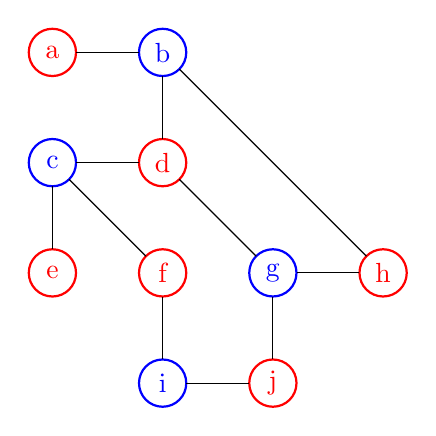
\begin{tikzpicture}
\tikzstyle{vertex}=[circle, inner sep=1pt,outer sep=0pt, 
	thick, node distance = 14mm,draw=black,minimum height=6mm,
]
\node[vertex,red] (a) { a };
\node[right of = a,vertex,blue] (b) { b };
\node[below of = a,vertex,blue] (c) { c };
\node[right of = c,vertex,red] (d) { d };
\node[below of = c,vertex,red] (e) { e };
\node[right of = e,vertex,red] (f) { f };
\node[right of = f,vertex,blue] (g) { g };
\node[right of = g,vertex,red] (h) { h };
\node[below of = f,vertex,blue] (i) { i };
\node[below of = g,vertex,red] (j) { j };
\path[-] (a) edge (b) ;
\path[-] (e) edge (c) ;
\path[-] (d) edge (c) ;
\path[-] (f) edge (c) ;
\path[-] (f) edge (i) ;
\path[-] (g) edge (h) ;
\path[-] (g) edge (j) ;
\path[-] (b) edge (d) ;
\path[-] (d) edge (g) ;
\path[-] (i) edge (j) ;
\path[-] (b) edge (h) ;

\end{tikzpicture}
}
\end{column}

\begin{column}{6cm}
\begin{itemize}
\item A graph is {\bf bipartite} if it can be colored with two colors such that every edge connects two nodes with different colors.
\end{itemize}
\end{column}
\end{columns}
\end{frame}

\begin{frame}
\frametitle{Bipartite graphs}
\begin{columns}
\begin{column}{5cm}
{\small \tt
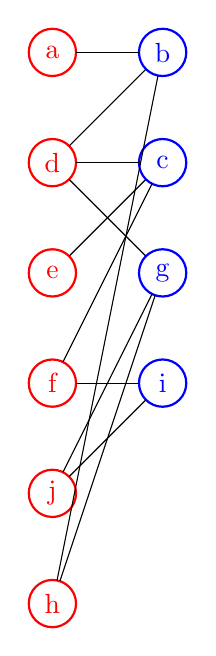
\begin{tikzpicture}
\tikzstyle{vertex}=[circle, inner sep=1pt,outer sep=0pt, 
	thick, node distance = 14mm,draw=black,minimum height=6mm,
]
\node[vertex,red] (a) { a };
\node[right of = a,vertex,blue] (b) { b };
\node[below of = b,vertex,blue] (c) { c };
\node[below of = a,vertex,red] (d) { d };
\node[below of = d,vertex,red] (e) { e };
\node[below of = e,vertex,red] (f) { f };
\node[below of = c,vertex,blue] (g) { g };
\node[below of = g,vertex,blue] (i) { i };
\node[below of = f,vertex,red] (j) { j };
\node[below of = j,vertex,red] (h) { h };
\path[-] (a) edge (b) ;
\path[-] (e) edge (c) ;
\path[-] (d) edge (c) ;
\path[-] (f) edge (c) ;
\path[-] (f) edge (i) ;
\path[-] (g) edge (h) ;
\path[-] (g) edge (j) ;
\path[-] (b) edge (d) ;
\path[-] (d) edge (g) ;
\path[-] (i) edge (j) ;
\path[-] (b) edge (h) ;

\end{tikzpicture}
}
\end{column}

\begin{column}{6cm}
\begin{itemize}
\item What could prevent a graph from being bipartite?
\end{itemize}
\end{column}
\end{columns}
\end{frame}

\begin{frame}
\frametitle{Bipartite graphs}
\begin{columns}
\begin{column}{5cm}
{\small \tt
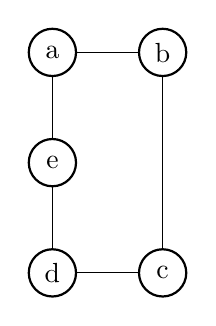
\begin{tikzpicture}
\tikzstyle{vertex}=[circle, inner sep=1pt,outer sep=0pt, 
	thick, node distance = 14mm,draw=black,minimum height=6mm,
]
\node[vertex] (a) { a };
\node[right of = a,vertex] (b) { b };
\node[below of = a,vertex] (e) { e };
\node[below of = e,vertex] (d) { d };
\node[right of = d,vertex] (c) { c };
\path[-] (a) edge (b) ;
\path[-] (e) edge (d) ;
\path[-] (d) edge (c) ;
\path[-] (b) edge (c) ;
\path[-] (e) edge (a) ;

\end{tikzpicture}
}
\end{column}

\begin{column}{6cm}
\begin{itemize}
\item A graph with a cycle with an odd length is impossible to color with two colors.
\end{itemize}
\end{column}
\end{columns}
\end{frame}

\begin{frame}
\frametitle{Characterizing bipartite graphs}
\begin{lemma}
\begin{itemize}
\item Let $G$ be a connected graph and $L_0, L_1, ..., L_k$ the layers of BFS.
\item Exactly one of the following is true for any $G$:
\begin{itemize}
\item[(1)] There is no edge between nodes in any $L_i$.
\item[(2)] There is an edge between nodes in some $L_i$.
\end{itemize}
In (1) $G$ is bipartite and in $(2)$ $G$ is not bipartite.
\end{itemize}
\end{lemma}

\begin{proof}
\begin{itemize}
\item First we show (1):
\begin{itemize}
\item Assume there is no edge $v-w$ such that $\{ v,w \} \subseteq L_i$
\item Color each node in an odd layer in one color and in even layers in the other.
\item Thus $G$ is bipartite.
\end{itemize}
\end{itemize}
\end{proof}
\end{frame}

\begin{frame}
\frametitle{Characterizing bipartite graphs}
\begin{lemma}
\begin{itemize}
\item Let $G$ be a connected graph and $L_0, L_1, ..., L_k$ the layers of BFS.
\item Exactly one of the following is true for any $G$:
\begin{itemize}
\item[(1)] There is no edge between nodes in any $L_i$.
\item[(2)] There is an edge between nodes in some $L_i$.
\end{itemize}
In (1) $G$ is bipartite and in $(2)$ $G$ is not bipartite.
\end{itemize}
\end{lemma}


\begin{proof}
\begin{itemize}
\item Second we show (2):
\begin{itemize}
\item We will show that (2) implies there is an odd length cycle in $G$.
\item Assume there is an edge $v-w$ such that $\{ v,w \} \subseteq L_j$.
\item Let $u$ be their lowest common ancestor and assume $u \in L_i$.
\item There is a cycle $u,...,v,w,...u$. The distance between $v$ and $w$ is $1$
\item The distance between $u$ and each of $v$ and $w$ is $j-i$
\item The total length of the cycle therefore is $1 + 2(j-i)$ which is odd.
\item Since $G$ contains an odd length cycle, $G$ is not bipartite.
% the corollary from wayne's slide
\end{itemize}
\end{itemize}
\end{proof}
\end{frame}

\begin{frame}
\frametitle{Directed graphs}
\begin{itemize}
\item Again $G = (V,E)$
\item An edge $e = (u,v)$ is from $u$ to $v$ 
\item Example directed graphs
\begin{itemize}
\item Links from one web page to another
\item Citation from journal article to another
\item Scheduling constraints in projects: some tasks must be performed before others
\end{itemize}
\item BFS: works naturally also for directed graphs
\end{itemize}
\end{frame}

\begin{frame}
\frametitle{Strong connectivity}
\begin{itemize}
\item Nodes $u$ and $v$ are {\bf mutually reachable} if there is a path from $u$ to $v$ and a path from $v$ to $u$
\item A directed graph is {\bf strongly connected} if every pair of nodes are mutually reachable
\end{itemize}
\begin{lemma}
Let $s$ be any node in $G$. $G$ is strongly connected $\iff$ every node is reachable from $s$ and $s$ is reachable from any node.
\end{lemma}


\begin{proof}
$\Rightarrow$ follows directly from the definition of strongly connected $G$. $\Leftarrow$ follows by constructing two paths:
\begin{itemize}
\item a path from $u$ to $v$ as $p = (u,...,s,...,v)$, and
\item a path from $v$ to $u$ as $q = (v,...,s,...,u)$.
\end{itemize}
\end{proof}
\end{frame}

\begin{frame}
\frametitle{Determining strong connectivity}
\begin{itemize}
\item Select any node $v \in V$
\item Use BFS on $G$ from $v$ and check if all of $V$ is reached
\item Construct $G^r$ from $G$ by reversing all edges
\item Use BFS on $G^r$ from $v$ and check if all of $V$ is reached
\item If all of $V$ is reached in both searches, $G$ is strongly connected
\item $O(n+m)$
\item We will next see Tarjan's algorithm which instead uses depth first search
and also lists all the strongly connected components
\end{itemize}
\end{frame}

\begin{frame}[fragile=singleslide]
\frametitle{Tarjan's Algorithm: Initial Processing of $0$}

\begin{columns}
\begin{column}{4cm}
{\tiny
\begin{tabbing}
\ahdr
\INT \>\ID{dfnum}\>\>\>\>\>\\
								\\
\PROC \CALL{strong\_connect}($v$)				\\
\>\CALL{dfn}($v$) \ASGN \ID{dfnum}				\\
\>\CALL{lowlink}($v$) \ASGN \ID{dfnum}				\\ 
\>\CALL{visited}($v$) \ASGN true				\\
\>\CALL{push}($v$) 						\\
\>\ID{dfnum} \ASGN \ID{dfnum} $ + 1$				\\
								\\
\>\FOR each $w \in succ(v)$ \DO	\\
\>\>\IF (\NOT \CALL{visited}($w$)) \{				\\
\>\>\>\CALL{strong\_connect}($w$)				\\
\>\>\>\CALL{lowlink}($v$) \ASGN \CALL{min}(\CALL{lowlink}($v$), \CALL{lowlink}($w$))\\
\>\>\} \ELIF (\CALL{dfn}($w$) $ < $ \CALL{dfn}($v$) \AND $w$ is on stack)\\
\>\>\>\CALL{lowlink}($v$) \ASGN \CALL{min}(\CALL{lowlink}($v$), \CALL{dfn}($w$))\\
\\
\>\IF (\CALL{lowlink}($v$) $=$ \CALL{dfn}($v$)) 		\\
\>\>\ID{scc} \ASGN \EMPTY					\\
\>\>\DO								\\
\>\>\>$w$ \ASGN \CALL{pop}()					\\
\>\>\>add $w$ to \ID{scc}					\\
\>\>\WHILE ($w \neq v$)						\\
\>\>\CALL{process\_scc}(\ID{scc})				\\
\END
\end{tabbing}
}

\end{column}
\begin{column}{4cm}
{\tiny
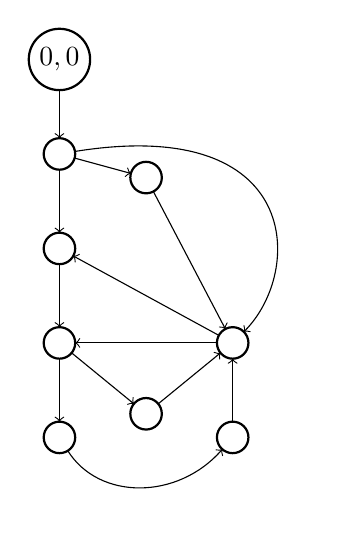
\begin{tikzpicture}
\tikzstyle{vertex}=[circle,thick, node distance = 12mm,
inner sep=2pt,outer sep=0pt,
draw=black,minimum height=4mm]
\node[vertex] at (0,0)	(0) { $0,0$ };
\node[vertex,below of =0,](1) {$$} ;
\node[vertex,below of =1,](2) {$$} ;
\node[vertex,below of =2,](3) {$$} ;
\node[vertex,below of =3,](4) {$$} ;
\node[vertex,right of =4,xshift=10mm](5) {$$} ;
\node[right of =4,xshift=-5mm,yshift=-8mm](5c1) {};
\node[right of =4,xshift=5mm,yshift=-8mm](5c2) {};
\node[vertex,above of =5,](6) {$$} ;
\node[vertex,right of =3,xshift=-1mm,yshift=-9mm](7) {$$} ;
\node[vertex,right of =2,xshift=-1mm,yshift=+9mm](8) {$$} ;

\node[right of =8,xshift=10mm,yshift=8mm](1c1) {};
\node[right of =8,xshift=10mm,yshift=-12mm](1c2) {};

\draw[->] (4) .. controls (5c1) and (5c2) ..  (5) ;
\draw[->] (1) .. controls (1c1) and (1c2) ..  (6) ;
\path[->] (0) edge (1) ;
\path[->] (1) edge (2) ;
\path[->] (1) edge (8) ;
\path[->] (8) edge (6) ;
\path[->] (2) edge (3) ;
\path[->] (3) edge (4) ;
\path[->] (5) edge (6) ;
\path[->] (3) edge (7) ;
\path[->] (7) edge (6) ;
\path[->] (6) edge (3) ;
\path[->] (6) edge (2) ;

\end{tikzpicture}
}
\end{column}
\begin{column}{1cm}
\begin{tabular}{|c|}
\hline
\\
\hline
\\
\hline
\\
\hline
\\
\hline
\\
\hline
\\
\hline
\\
\hline
\\
\hline
$0$\\
\hline
\end{tabular}\\
stack
\end{column}
\end{columns}
\end{frame}




\begin{frame}[fragile=singleslide]
\frametitle{Tarjan's Algorithm: Initial Processing of $1$}

\begin{columns}
\begin{column}{4cm}
{\tiny
\begin{tabbing}
\ahdr
\INT \>\ID{dfnum}\>\>\>\>\>\\
								\\
\PROC \CALL{strong\_connect}($v$)				\\
\>\CALL{dfn}($v$) \ASGN \ID{dfnum}				\\
\>\CALL{lowlink}($v$) \ASGN \ID{dfnum}				\\ 
\>\CALL{visited}($v$) \ASGN true				\\
\>\CALL{push}($v$) 						\\
\>\ID{dfnum} \ASGN \ID{dfnum} $ + 1$				\\
								\\
\>\FOR each $w \in succ(v)$ \DO	\\
\>\>\IF (\NOT \CALL{visited}($w$)) \{				\\
\>\>\>\CALL{strong\_connect}($w$)				\\
\>\>\>\CALL{lowlink}($v$) \ASGN \CALL{min}(\CALL{lowlink}($v$), \CALL{lowlink}($w$))\\
\>\>\} \ELIF (\CALL{dfn}($w$) $ < $ \CALL{dfn}($v$) \AND $w$ is on stack)\\
\>\>\>\CALL{lowlink}($v$) \ASGN \CALL{min}(\CALL{lowlink}($v$), \CALL{dfn}($w$))\\
\\
\>\IF (\CALL{lowlink}($v$) $=$ \CALL{dfn}($v$)) 		\\
\>\>\ID{scc} \ASGN \EMPTY					\\
\>\>\DO								\\
\>\>\>$w$ \ASGN \CALL{pop}()					\\
\>\>\>add $w$ to \ID{scc}					\\
\>\>\WHILE ($w \neq v$)						\\
\>\>\CALL{process\_scc}(\ID{scc})				\\
\END
\end{tabbing}
}

\end{column}
\begin{column}{4cm}
{\tiny
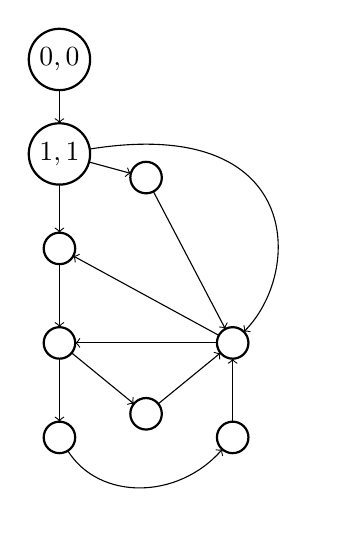
\begin{tikzpicture}
\tikzstyle{vertex}=[circle,thick, node distance = 12mm,
inner sep=2pt,outer sep=0pt,
draw=black,minimum height=4mm]
\node[vertex] at (0,0)	(0) { $0,0$ };
\node[vertex,below of =0,](1) {$1,1$} ;
\node[vertex,below of =1,](2) {$$} ;
\node[vertex,below of =2,](3) {$$} ;
\node[vertex,below of =3,](4) {$$} ;
\node[vertex,right of =4,xshift=10mm](5) {$$} ;
\node[right of =4,xshift=-5mm,yshift=-8mm](5c1) {};
\node[right of =4,xshift=5mm,yshift=-8mm](5c2) {};
\node[vertex,above of =5,](6) {$$} ;
\node[vertex,right of =3,xshift=-1mm,yshift=-9mm](7) {$$} ;
\node[vertex,right of =2,xshift=-1mm,yshift=+9mm](8) {$$} ;

\node[right of =8,xshift=10mm,yshift=8mm](1c1) {};
\node[right of =8,xshift=10mm,yshift=-12mm](1c2) {};

\draw[->] (4) .. controls (5c1) and (5c2) ..  (5) ;
\draw[->] (1) .. controls (1c1) and (1c2) ..  (6) ;
\path[->] (0) edge (1) ;
\path[->] (1) edge (2) ;
\path[->] (1) edge (8) ;
\path[->] (8) edge (6) ;
\path[->] (2) edge (3) ;
\path[->] (3) edge (4) ;
\path[->] (5) edge (6) ;
\path[->] (3) edge (7) ;
\path[->] (7) edge (6) ;
\path[->] (6) edge (3) ;
\path[->] (6) edge (2) ;

\end{tikzpicture}
}
\end{column}
\begin{column}{1cm}
\begin{tabular}{|c|}
\hline
\\
\hline
\\
\hline
\\
\hline
\\
\hline
\\
\hline
\\
\hline
\\
\hline
$1$\\
\hline
$0$\\
\hline
\end{tabular}\\
stack
\end{column}
\end{columns}
\end{frame}







\begin{frame}[fragile=singleslide]
\frametitle{Tarjan's Algorithm: Initial Processing of $2$}

\begin{columns}
\begin{column}{4cm}
{\tiny
\begin{tabbing}
\ahdr
\INT \>\ID{dfnum}\>\>\>\>\>\\
								\\
\PROC \CALL{strong\_connect}($v$)				\\
\>\CALL{dfn}($v$) \ASGN \ID{dfnum}				\\
\>\CALL{lowlink}($v$) \ASGN \ID{dfnum}				\\ 
\>\CALL{visited}($v$) \ASGN true				\\
\>\CALL{push}($v$) 						\\
\>\ID{dfnum} \ASGN \ID{dfnum} $ + 1$				\\
								\\
\>\FOR each $w \in succ(v)$ \DO	\\
\>\>\IF (\NOT \CALL{visited}($w$)) \{				\\
\>\>\>\CALL{strong\_connect}($w$)				\\
\>\>\>\CALL{lowlink}($v$) \ASGN \CALL{min}(\CALL{lowlink}($v$), \CALL{lowlink}($w$))\\
\>\>\} \ELIF (\CALL{dfn}($w$) $ < $ \CALL{dfn}($v$) \AND $w$ is on stack)\\
\>\>\>\CALL{lowlink}($v$) \ASGN \CALL{min}(\CALL{lowlink}($v$), \CALL{dfn}($w$))\\
\\
\>\IF (\CALL{lowlink}($v$) $=$ \CALL{dfn}($v$)) 		\\
\>\>\ID{scc} \ASGN \EMPTY					\\
\>\>\DO								\\
\>\>\>$w$ \ASGN \CALL{pop}()					\\
\>\>\>add $w$ to \ID{scc}					\\
\>\>\WHILE ($w \neq v$)						\\
\>\>\CALL{process\_scc}(\ID{scc})				\\
\END
\end{tabbing}
}

\end{column}
\begin{column}{4cm}
{\tiny
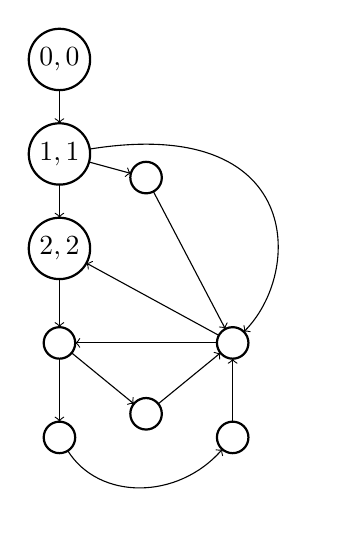
\begin{tikzpicture}
\tikzstyle{vertex}=[circle,thick, node distance = 12mm,
inner sep=2pt,outer sep=0pt,
draw=black,minimum height=4mm]
\node[vertex] at (0,0)	(0) { $0,0$ };
\node[vertex,below of =0,](1) {$1,1$} ;
\node[vertex,below of =1,](2) {$2,2$} ;
\node[vertex,below of =2,](3) {$$} ;
\node[vertex,below of =3,](4) {$$} ;
\node[vertex,right of =4,xshift=10mm](5) {$$} ;
\node[right of =4,xshift=-5mm,yshift=-8mm](5c1) {};
\node[right of =4,xshift=5mm,yshift=-8mm](5c2) {};
\node[vertex,above of =5,](6) {$$} ;
\node[vertex,right of =3,xshift=-1mm,yshift=-9mm](7) {$$} ;
\node[vertex,right of =2,xshift=-1mm,yshift=+9mm](8) {$$} ;

\node[right of =8,xshift=10mm,yshift=8mm](1c1) {};
\node[right of =8,xshift=10mm,yshift=-12mm](1c2) {};

\draw[->] (4) .. controls (5c1) and (5c2) ..  (5) ;
\draw[->] (1) .. controls (1c1) and (1c2) ..  (6) ;
\path[->] (0) edge (1) ;
\path[->] (1) edge (2) ;
\path[->] (1) edge (8) ;
\path[->] (8) edge (6) ;
\path[->] (2) edge (3) ;
\path[->] (3) edge (4) ;
\path[->] (5) edge (6) ;
\path[->] (3) edge (7) ;
\path[->] (7) edge (6) ;
\path[->] (6) edge (3) ;
\path[->] (6) edge (2) ;

\end{tikzpicture}
}
\end{column}
\begin{column}{1cm}
\begin{tabular}{|c|}
\hline
\\
\hline
\\
\hline
\\
\hline
\\
\hline
\\
\hline
\\
\hline
$2$\\
\hline
$1$\\
\hline
$0$\\
\hline
\end{tabular}\\
stack
\end{column}
\end{columns}
\end{frame}





% @@

\begin{frame}[fragile=singleslide]
\frametitle{Tarjan's Algorithm: Initial Processing of $3$}

\begin{columns}
\begin{column}{4cm}
{\tiny
\begin{tabbing}
\ahdr
\INT \>\ID{dfnum}\>\>\>\>\>\\
								\\
\PROC \CALL{strong\_connect}($v$)				\\
\>\CALL{dfn}($v$) \ASGN \ID{dfnum}				\\
\>\CALL{lowlink}($v$) \ASGN \ID{dfnum}				\\ 
\>\CALL{visited}($v$) \ASGN true				\\
\>\CALL{push}($v$) 						\\
\>\ID{dfnum} \ASGN \ID{dfnum} $ + 1$				\\
								\\
\>\FOR each $w \in succ(v)$ \DO	\\
\>\>\IF (\NOT \CALL{visited}($w$)) \{				\\
\>\>\>\CALL{strong\_connect}($w$)				\\
\>\>\>\CALL{lowlink}($v$) \ASGN \CALL{min}(\CALL{lowlink}($v$), \CALL{lowlink}($w$))\\
\>\>\} \ELIF (\CALL{dfn}($w$) $ < $ \CALL{dfn}($v$) \AND $w$ is on stack)\\
\>\>\>\CALL{lowlink}($v$) \ASGN \CALL{min}(\CALL{lowlink}($v$), \CALL{dfn}($w$))\\
\\
\>\IF (\CALL{lowlink}($v$) $=$ \CALL{dfn}($v$)) 		\\
\>\>\ID{scc} \ASGN \EMPTY					\\
\>\>\DO								\\
\>\>\>$w$ \ASGN \CALL{pop}()					\\
\>\>\>add $w$ to \ID{scc}					\\
\>\>\WHILE ($w \neq v$)						\\
\>\>\CALL{process\_scc}(\ID{scc})				\\
\END
\end{tabbing}
}

\end{column}
\begin{column}{4cm}
{\tiny
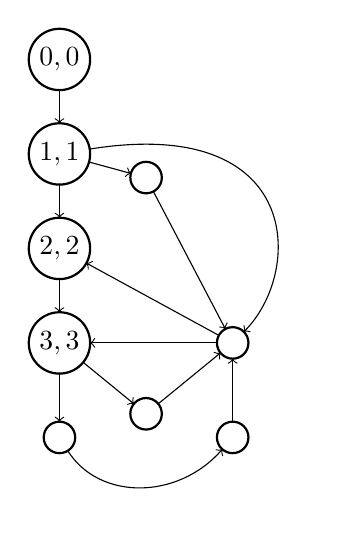
\begin{tikzpicture}
\tikzstyle{vertex}=[circle,thick, node distance = 12mm,
inner sep=2pt,outer sep=0pt,
draw=black,minimum height=4mm]
\node[vertex] at (0,0)	(0) { $0,0$ };
\node[vertex,below of =0,](1) {$1,1$} ;
\node[vertex,below of =1,](2) {$2,2$} ;
\node[vertex,below of =2,](3) {$3,3$} ;
\node[vertex,below of =3,](4) {$$} ;
\node[vertex,right of =4,xshift=10mm](5) {$$} ;
\node[right of =4,xshift=-5mm,yshift=-8mm](5c1) {};
\node[right of =4,xshift=5mm,yshift=-8mm](5c2) {};
\node[vertex,above of =5,](6) {$$} ;
\node[vertex,right of =3,xshift=-1mm,yshift=-9mm](7) {$$} ;
\node[vertex,right of =2,xshift=-1mm,yshift=+9mm](8) {$$} ;

\node[right of =8,xshift=10mm,yshift=8mm](1c1) {};
\node[right of =8,xshift=10mm,yshift=-12mm](1c2) {};

\draw[->] (4) .. controls (5c1) and (5c2) ..  (5) ;
\draw[->] (1) .. controls (1c1) and (1c2) ..  (6) ;
\path[->] (0) edge (1) ;
\path[->] (1) edge (2) ;
\path[->] (1) edge (8) ;
\path[->] (8) edge (6) ;
\path[->] (2) edge (3) ;
\path[->] (3) edge (4) ;
\path[->] (5) edge (6) ;
\path[->] (3) edge (7) ;
\path[->] (7) edge (6) ;
\path[->] (6) edge (3) ;
\path[->] (6) edge (2) ;

\end{tikzpicture}
}
\end{column}
\begin{column}{1cm}
\begin{tabular}{|c|}
\hline
\\
\hline
\\
\hline
\\
\hline
\\
\hline
\\
\hline
$3$\\
\hline
$2$\\
\hline
$1$\\
\hline
$0$\\
\hline
\end{tabular}\\
stack
\end{column}
\end{columns}
\end{frame}




% @@

\begin{frame}[fragile=singleslide]
\frametitle{Tarjan's Algorithm: Initial Processing of $4$}

\begin{columns}
\begin{column}{4cm}
{\tiny
\begin{tabbing}
\ahdr
\INT \>\ID{dfnum}\>\>\>\>\>\\
								\\
\PROC \CALL{strong\_connect}($v$)				\\
\>\CALL{dfn}($v$) \ASGN \ID{dfnum}				\\
\>\CALL{lowlink}($v$) \ASGN \ID{dfnum}				\\ 
\>\CALL{visited}($v$) \ASGN true				\\
\>\CALL{push}($v$) 						\\
\>\ID{dfnum} \ASGN \ID{dfnum} $ + 1$				\\
								\\
\>\FOR each $w \in succ(v)$ \DO	\\
\>\>\IF (\NOT \CALL{visited}($w$)) \{				\\
\>\>\>\CALL{strong\_connect}($w$)				\\
\>\>\>\CALL{lowlink}($v$) \ASGN \CALL{min}(\CALL{lowlink}($v$), \CALL{lowlink}($w$))\\
\>\>\} \ELIF (\CALL{dfn}($w$) $ < $ \CALL{dfn}($v$) \AND $w$ is on stack)\\
\>\>\>\CALL{lowlink}($v$) \ASGN \CALL{min}(\CALL{lowlink}($v$), \CALL{dfn}($w$))\\
\\
\>\IF (\CALL{lowlink}($v$) $=$ \CALL{dfn}($v$)) 		\\
\>\>\ID{scc} \ASGN \EMPTY					\\
\>\>\DO								\\
\>\>\>$w$ \ASGN \CALL{pop}()					\\
\>\>\>add $w$ to \ID{scc}					\\
\>\>\WHILE ($w \neq v$)						\\
\>\>\CALL{process\_scc}(\ID{scc})				\\
\END
\end{tabbing}
}

\end{column}
\begin{column}{4cm}
{\tiny
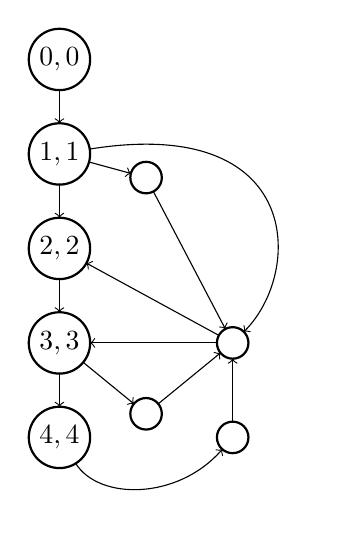
\begin{tikzpicture}
\tikzstyle{vertex}=[circle,thick, node distance = 12mm,
inner sep=2pt,outer sep=0pt,
draw=black,minimum height=4mm]
\node[vertex] at (0,0)	(0) { $0,0$ };
\node[vertex,below of =0,](1) {$1,1$} ;
\node[vertex,below of =1,](2) {$2,2$} ;
\node[vertex,below of =2,](3) {$3,3$} ;
\node[vertex,below of =3,](4) {$4,4$} ;
\node[vertex,right of =4,xshift=10mm](5) {$$} ;
\node[right of =4,xshift=-5mm,yshift=-8mm](5c1) {};
\node[right of =4,xshift=5mm,yshift=-8mm](5c2) {};
\node[vertex,above of =5,](6) {$$} ;
\node[vertex,right of =3,xshift=-1mm,yshift=-9mm](7) {$$} ;
\node[vertex,right of =2,xshift=-1mm,yshift=+9mm](8) {$$} ;

\node[right of =8,xshift=10mm,yshift=8mm](1c1) {};
\node[right of =8,xshift=10mm,yshift=-12mm](1c2) {};

\draw[->] (4) .. controls (5c1) and (5c2) ..  (5) ;
\draw[->] (1) .. controls (1c1) and (1c2) ..  (6) ;
\path[->] (0) edge (1) ;
\path[->] (1) edge (2) ;
\path[->] (1) edge (8) ;
\path[->] (8) edge (6) ;
\path[->] (2) edge (3) ;
\path[->] (3) edge (4) ;
\path[->] (5) edge (6) ;
\path[->] (3) edge (7) ;
\path[->] (7) edge (6) ;
\path[->] (6) edge (3) ;
\path[->] (6) edge (2) ;

\end{tikzpicture}
}
\end{column}
\begin{column}{1cm}
\begin{tabular}{|c|}
\hline
\\
\hline
\\
\hline
\\
\hline
\\
\hline
$4$\\
\hline
$3$\\
\hline
$2$\\
\hline
$1$\\
\hline
$0$\\
\hline
\end{tabular}\\
stack
\end{column}
\end{columns}
\end{frame}




% @@

\begin{frame}[fragile=singleslide]
\frametitle{Tarjan's Algorithm: Initial Processing of $5$}

\begin{columns}
\begin{column}{4cm}
{\tiny
\begin{tabbing}
\ahdr
\INT \>\ID{dfnum}\>\>\>\>\>\\
								\\
\PROC \CALL{strong\_connect}($v$)				\\
\>\CALL{dfn}($v$) \ASGN \ID{dfnum}				\\
\>\CALL{lowlink}($v$) \ASGN \ID{dfnum}				\\ 
\>\CALL{visited}($v$) \ASGN true				\\
\>\CALL{push}($v$) 						\\
\>\ID{dfnum} \ASGN \ID{dfnum} $ + 1$				\\
								\\
\>\FOR each $w \in succ(v)$ \DO	\\
\>\>\IF (\NOT \CALL{visited}($w$)) \{				\\
\>\>\>\CALL{strong\_connect}($w$)				\\
\>\>\>\CALL{lowlink}($v$) \ASGN \CALL{min}(\CALL{lowlink}($v$), \CALL{lowlink}($w$))\\
\>\>\} \ELIF (\CALL{dfn}($w$) $ < $ \CALL{dfn}($v$) \AND $w$ is on stack)\\
\>\>\>\CALL{lowlink}($v$) \ASGN \CALL{min}(\CALL{lowlink}($v$), \CALL{dfn}($w$))\\
\\
\>\IF (\CALL{lowlink}($v$) $=$ \CALL{dfn}($v$)) 		\\
\>\>\ID{scc} \ASGN \EMPTY					\\
\>\>\DO								\\
\>\>\>$w$ \ASGN \CALL{pop}()					\\
\>\>\>add $w$ to \ID{scc}					\\
\>\>\WHILE ($w \neq v$)						\\
\>\>\CALL{process\_scc}(\ID{scc})				\\
\END
\end{tabbing}
}

\end{column}
\begin{column}{4cm}
{\tiny
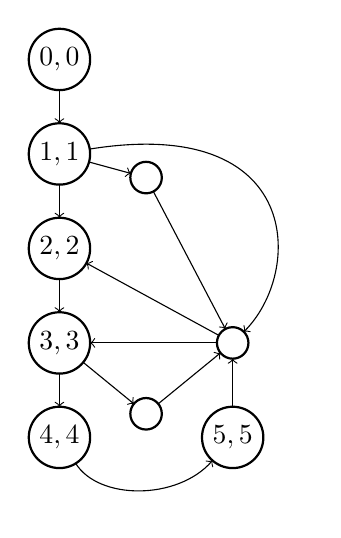
\begin{tikzpicture}
\tikzstyle{vertex}=[circle,thick, node distance = 12mm,
inner sep=2pt,outer sep=0pt,
draw=black,minimum height=4mm]
\node[vertex] at (0,0)	(0) { $0,0$ };
\node[vertex,below of =0,](1) {$1,1$} ;
\node[vertex,below of =1,](2) {$2,2$} ;
\node[vertex,below of =2,](3) {$3,3$} ;
\node[vertex,below of =3,](4) {$4,4$} ;
\node[vertex,right of =4,xshift=10mm](5) {$5,5$} ;
\node[right of =4,xshift=-5mm,yshift=-8mm](5c1) {};
\node[right of =4,xshift=5mm,yshift=-8mm](5c2) {};
\node[vertex,above of =5,](6) {$$} ;
\node[vertex,right of =3,xshift=-1mm,yshift=-9mm](7) {$$} ;
\node[vertex,right of =2,xshift=-1mm,yshift=+9mm](8) {$$} ;

\node[right of =8,xshift=10mm,yshift=8mm](1c1) {};
\node[right of =8,xshift=10mm,yshift=-12mm](1c2) {};

\draw[->] (4) .. controls (5c1) and (5c2) ..  (5) ;
\draw[->] (1) .. controls (1c1) and (1c2) ..  (6) ;
\path[->] (0) edge (1) ;
\path[->] (1) edge (2) ;
\path[->] (1) edge (8) ;
\path[->] (8) edge (6) ;
\path[->] (2) edge (3) ;
\path[->] (3) edge (4) ;
\path[->] (5) edge (6) ;
\path[->] (3) edge (7) ;
\path[->] (7) edge (6) ;
\path[->] (6) edge (3) ;
\path[->] (6) edge (2) ;

\end{tikzpicture}
}
\end{column}
\begin{column}{1cm}
\begin{tabular}{|c|}
\hline
\\
\hline
\\
\hline
\\
\hline
$5$\\
\hline
$4$\\
\hline
$3$\\
\hline
$2$\\
\hline
$1$\\
\hline
$0$\\
\hline
\end{tabular}\\
stack
\end{column}
\end{columns}
\end{frame}




% @@

\begin{frame}[fragile=singleslide]
\frametitle{Tarjan's Algorithm: Initial Processing of $6$}

\begin{columns}
\begin{column}{4cm}
{\tiny
\begin{tabbing}
\ahdr
\INT \>\ID{dfnum}\>\>\>\>\>\\
								\\
\PROC \CALL{strong\_connect}($v$)				\\
\>\CALL{dfn}($v$) \ASGN \ID{dfnum}				\\
\>\CALL{lowlink}($v$) \ASGN \ID{dfnum}				\\ 
\>\CALL{visited}($v$) \ASGN true				\\
\>\CALL{push}($v$) 						\\
\>\ID{dfnum} \ASGN \ID{dfnum} $ + 1$				\\
								\\
\>\FOR each $w \in succ(v)$ \DO	\\
\>\>\IF (\NOT \CALL{visited}($w$)) \{				\\
\>\>\>\CALL{strong\_connect}($w$)				\\
\>\>\>\CALL{lowlink}($v$) \ASGN \CALL{min}(\CALL{lowlink}($v$), \CALL{lowlink}($w$))\\
\>\>\} \ELIF (\CALL{dfn}($w$) $ < $ \CALL{dfn}($v$) \AND $w$ is on stack)\\
\>\>\>\CALL{lowlink}($v$) \ASGN \CALL{min}(\CALL{lowlink}($v$), \CALL{dfn}($w$))\\
\\
\>\IF (\CALL{lowlink}($v$) $=$ \CALL{dfn}($v$)) 		\\
\>\>\ID{scc} \ASGN \EMPTY					\\
\>\>\DO								\\
\>\>\>$w$ \ASGN \CALL{pop}()					\\
\>\>\>add $w$ to \ID{scc}					\\
\>\>\WHILE ($w \neq v$)						\\
\>\>\CALL{process\_scc}(\ID{scc})				\\
\END
\end{tabbing}
}

\end{column}
\begin{column}{4cm}
{\tiny
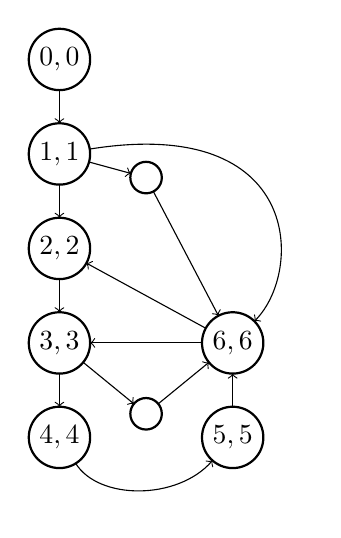
\begin{tikzpicture}
\tikzstyle{vertex}=[circle,thick, node distance = 12mm,
inner sep=2pt,outer sep=0pt,
draw=black,minimum height=4mm]
\node[vertex] at (0,0)	(0) { $0,0$ };
\node[vertex,below of =0,](1) {$1,1$} ;
\node[vertex,below of =1,](2) {$2,2$} ;
\node[vertex,below of =2,](3) {$3,3$} ;
\node[vertex,below of =3,](4) {$4,4$} ;
\node[vertex,right of =4,xshift=10mm](5) {$5,5$} ;
\node[right of =4,xshift=-5mm,yshift=-8mm](5c1) {};
\node[right of =4,xshift=5mm,yshift=-8mm](5c2) {};
\node[vertex,above of =5,](6) {$6,6$} ;
\node[vertex,right of =3,xshift=-1mm,yshift=-9mm](7) {$$} ;
\node[vertex,right of =2,xshift=-1mm,yshift=+9mm](8) {$$} ;

\node[right of =8,xshift=10mm,yshift=8mm](1c1) {};
\node[right of =8,xshift=10mm,yshift=-12mm](1c2) {};

\draw[->] (4) .. controls (5c1) and (5c2) ..  (5) ;
\draw[->] (1) .. controls (1c1) and (1c2) ..  (6) ;
\path[->] (0) edge (1) ;
\path[->] (1) edge (2) ;
\path[->] (1) edge (8) ;
\path[->] (8) edge (6) ;
\path[->] (2) edge (3) ;
\path[->] (3) edge (4) ;
\path[->] (5) edge (6) ;
\path[->] (3) edge (7) ;
\path[->] (7) edge (6) ;
\path[->] (6) edge (3) ;
\path[->] (6) edge (2) ;

\end{tikzpicture}
}
\end{column}
\begin{column}{1cm}
\begin{tabular}{|c|}
\hline
\\
\hline
\\
\hline
$6$\\
\hline
$5$\\
\hline
$4$\\
\hline
$3$\\
\hline
$2$\\
\hline
$1$\\
\hline
$0$\\
\hline
\end{tabular}\\
stack
\end{column}
\end{columns}
\end{frame}




% @@

\begin{frame}[fragile=singleslide]
\frametitle{Tarjan's Algorithm: More Processing of $6$}

\begin{columns}
\begin{column}{4cm}
{\tiny
\begin{itemize}
\item $(6,2) \Rightarrow 6$ in same scc as $2$. 
\end{itemize}

\begin{tabbing}
\ahdr
\INT \>\ID{dfnum}\>\>\>\>\>\\
								\\
\PROC \CALL{strong\_connect}($v$)				\\
\>\CALL{dfn}($v$) \ASGN \ID{dfnum}				\\
\>\CALL{lowlink}($v$) \ASGN \ID{dfnum}				\\ 
\>\CALL{visited}($v$) \ASGN true				\\
\>\CALL{push}($v$) 						\\
\>\ID{dfnum} \ASGN \ID{dfnum} $ + 1$				\\
								\\
\>\FOR each $w \in succ(v)$ \DO	\\
\>\>\IF (\NOT \CALL{visited}($w$)) \{				\\
\>\>\>\CALL{strong\_connect}($w$)				\\
\>\>\>\CALL{lowlink}($v$) \ASGN \CALL{min}(\CALL{lowlink}($v$), \CALL{lowlink}($w$))\\
\>\>\} \ELIF (\CALL{dfn}($w$) $ < $ \CALL{dfn}($v$) \AND $w$ is on stack)\\
\>\>\>\CALL{lowlink}($v$) \ASGN \CALL{min}(\CALL{lowlink}($v$), \CALL{dfn}($w$))\\
\\
\>\IF (\CALL{lowlink}($v$) $=$ \CALL{dfn}($v$)) 		\\
\>\>\ID{scc} \ASGN \EMPTY					\\
\>\>\DO								\\
\>\>\>$w$ \ASGN \CALL{pop}()					\\
\>\>\>add $w$ to \ID{scc}					\\
\>\>\WHILE ($w \neq v$)						\\
\>\>\CALL{process\_scc}(\ID{scc})				\\
\END
\end{tabbing}
}

\end{column}
\begin{column}{4cm}
{\tiny
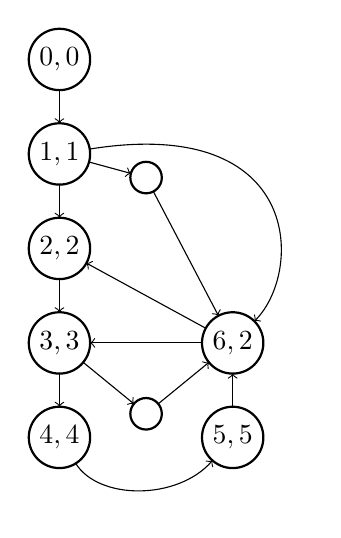
\begin{tikzpicture}
\tikzstyle{vertex}=[circle,thick, node distance = 12mm,
inner sep=2pt,outer sep=0pt,
draw=black,minimum height=4mm]
\node[vertex] at (0,0)	(0) { $0,0$ };
\node[vertex,below of =0,](1) {$1,1$} ;
\node[vertex,below of =1,](2) {$2,2$} ;
\node[vertex,below of =2,](3) {$3,3$} ;
\node[vertex,below of =3,](4) {$4,4$} ;
\node[vertex,right of =4,xshift=10mm](5) {$5,5$} ;
\node[right of =4,xshift=-5mm,yshift=-8mm](5c1) {};
\node[right of =4,xshift=5mm,yshift=-8mm](5c2) {};
\node[vertex,above of =5,](6) {$6,2$} ;
\node[vertex,right of =3,xshift=-1mm,yshift=-9mm](7) {$$} ;
\node[vertex,right of =2,xshift=-1mm,yshift=+9mm](8) {$$} ;

\node[right of =8,xshift=10mm,yshift=8mm](1c1) {};
\node[right of =8,xshift=10mm,yshift=-12mm](1c2) {};

\draw[->] (4) .. controls (5c1) and (5c2) ..  (5) ;
\draw[->] (1) .. controls (1c1) and (1c2) ..  (6) ;
\path[->] (0) edge (1) ;
\path[->] (1) edge (2) ;
\path[->] (1) edge (8) ;
\path[->] (8) edge (6) ;
\path[->] (2) edge (3) ;
\path[->] (3) edge (4) ;
\path[->] (5) edge (6) ;
\path[->] (3) edge (7) ;
\path[->] (7) edge (6) ;
\path[->] (6) edge (3) ;
\path[->] (6) edge (2) ;

\end{tikzpicture}
}
\end{column}
\begin{column}{1cm}
\begin{tabular}{|c|}
\hline
\\
\hline
\\
\hline
$6$\\
\hline
$5$\\
\hline
$4$\\
\hline
$3$\\
\hline
$2$\\
\hline
$1$\\
\hline
$0$\\
\hline
\end{tabular}\\
stack
\end{column}
\end{columns}
\end{frame}




% @@

\begin{frame}[fragile=singleslide]
\frametitle{Tarjan's Algorithm: More Processing of $6$}

\begin{columns}
\begin{column}{4cm}
{\tiny
\begin{itemize}
\item $(6,3)$. no action.
\end{itemize}

\begin{tabbing}
\ahdr
\INT \>\ID{dfnum}\>\>\>\>\>\\
								\\
\PROC \CALL{strong\_connect}($v$)				\\
\>\CALL{dfn}($v$) \ASGN \ID{dfnum}				\\
\>\CALL{lowlink}($v$) \ASGN \ID{dfnum}				\\ 
\>\CALL{visited}($v$) \ASGN true				\\
\>\CALL{push}($v$) 						\\
\>\ID{dfnum} \ASGN \ID{dfnum} $ + 1$				\\
								\\
\>\FOR each $w \in succ(v)$ \DO	\\
\>\>\IF (\NOT \CALL{visited}($w$)) \{				\\
\>\>\>\CALL{strong\_connect}($w$)				\\
\>\>\>\CALL{lowlink}($v$) \ASGN \CALL{min}(\CALL{lowlink}($v$), \CALL{lowlink}($w$))\\
\>\>\} \ELIF (\CALL{dfn}($w$) $ < $ \CALL{dfn}($v$) \AND $w$ is on stack)\\
\>\>\>\CALL{lowlink}($v$) \ASGN \CALL{min}(\CALL{lowlink}($v$), \CALL{dfn}($w$))\\
\\
\>\IF (\CALL{lowlink}($v$) $=$ \CALL{dfn}($v$)) 		\\
\>\>\ID{scc} \ASGN \EMPTY					\\
\>\>\DO								\\
\>\>\>$w$ \ASGN \CALL{pop}()					\\
\>\>\>add $w$ to \ID{scc}					\\
\>\>\WHILE ($w \neq v$)						\\
\>\>\CALL{process\_scc}(\ID{scc})				\\
\END
\end{tabbing}
}

\end{column}
\begin{column}{4cm}
{\tiny
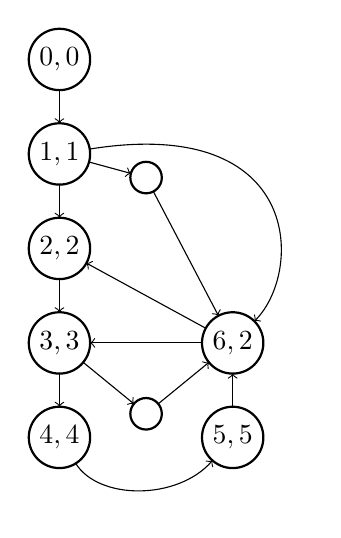
\begin{tikzpicture}
\tikzstyle{vertex}=[circle,thick, node distance = 12mm,
inner sep=2pt,outer sep=0pt,
draw=black,minimum height=4mm]
\node[vertex] at (0,0)	(0) { $0,0$ };
\node[vertex,below of =0,](1) {$1,1$} ;
\node[vertex,below of =1,](2) {$2,2$} ;
\node[vertex,below of =2,](3) {$3,3$} ;
\node[vertex,below of =3,](4) {$4,4$} ;
\node[vertex,right of =4,xshift=10mm](5) {$5,5$} ;
\node[right of =4,xshift=-5mm,yshift=-8mm](5c1) {};
\node[right of =4,xshift=5mm,yshift=-8mm](5c2) {};
\node[vertex,above of =5,](6) {$6,2$} ;
\node[vertex,right of =3,xshift=-1mm,yshift=-9mm](7) {$$} ;
\node[vertex,right of =2,xshift=-1mm,yshift=+9mm](8) {$$} ;

\node[right of =8,xshift=10mm,yshift=8mm](1c1) {};
\node[right of =8,xshift=10mm,yshift=-12mm](1c2) {};

\draw[->] (4) .. controls (5c1) and (5c2) ..  (5) ;
\draw[->] (1) .. controls (1c1) and (1c2) ..  (6) ;
\path[->] (0) edge (1) ;
\path[->] (1) edge (2) ;
\path[->] (1) edge (8) ;
\path[->] (8) edge (6) ;
\path[->] (2) edge (3) ;
\path[->] (3) edge (4) ;
\path[->] (5) edge (6) ;
\path[->] (3) edge (7) ;
\path[->] (7) edge (6) ;
\path[->] (6) edge (3) ;
\path[->] (6) edge (2) ;

\end{tikzpicture}
}
\end{column}
\begin{column}{1cm}
\begin{tabular}{|c|}
\hline
\\
\hline
\\
\hline
$6$\\
\hline
$5$\\
\hline
$4$\\
\hline
$3$\\
\hline
$2$\\
\hline
$1$\\
\hline
$0$\\
\hline
\end{tabular}\\
stack
\end{column}
\end{columns}
\end{frame}




% @@

\begin{frame}[fragile=singleslide]
\frametitle{Tarjan's Algorithm: More Processing of $6$}

\begin{columns}
\begin{column}{4cm}
{\tiny
\begin{itemize}
\item $6$ remains on the stack.
\end{itemize}

\begin{tabbing}
\ahdr
\INT \>\ID{dfnum}\>\>\>\>\>\\
								\\
\PROC \CALL{strong\_connect}($v$)				\\
\>\CALL{dfn}($v$) \ASGN \ID{dfnum}				\\
\>\CALL{lowlink}($v$) \ASGN \ID{dfnum}				\\ 
\>\CALL{visited}($v$) \ASGN true				\\
\>\CALL{push}($v$) 						\\
\>\ID{dfnum} \ASGN \ID{dfnum} $ + 1$				\\
								\\
\>\FOR each $w \in succ(v)$ \DO	\\
\>\>\IF (\NOT \CALL{visited}($w$)) \{				\\
\>\>\>\CALL{strong\_connect}($w$)				\\
\>\>\>\CALL{lowlink}($v$) \ASGN \CALL{min}(\CALL{lowlink}($v$), \CALL{lowlink}($w$))\\
\>\>\} \ELIF (\CALL{dfn}($w$) $ < $ \CALL{dfn}($v$) \AND $w$ is on stack)\\
\>\>\>\CALL{lowlink}($v$) \ASGN \CALL{min}(\CALL{lowlink}($v$), \CALL{dfn}($w$))\\
\\
\>\IF (\CALL{lowlink}($v$) $=$ \CALL{dfn}($v$)) 		\\
\>\>\ID{scc} \ASGN \EMPTY					\\
\>\>\DO								\\
\>\>\>$w$ \ASGN \CALL{pop}()					\\
\>\>\>add $w$ to \ID{scc}					\\
\>\>\WHILE ($w \neq v$)						\\
\>\>\CALL{process\_scc}(\ID{scc})				\\
\END
\end{tabbing}
}

\end{column}
\begin{column}{4cm}
{\tiny
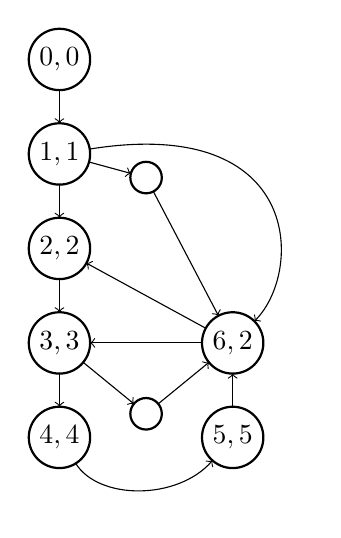
\begin{tikzpicture}
\tikzstyle{vertex}=[circle,thick, node distance = 12mm,
inner sep=2pt,outer sep=0pt,
draw=black,minimum height=4mm]
\node[vertex] at (0,0)	(0) { $0,0$ };
\node[vertex,below of =0,](1) {$1,1$} ;
\node[vertex,below of =1,](2) {$2,2$} ;
\node[vertex,below of =2,](3) {$3,3$} ;
\node[vertex,below of =3,](4) {$4,4$} ;
\node[vertex,right of =4,xshift=10mm](5) {$5,5$} ;
\node[right of =4,xshift=-5mm,yshift=-8mm](5c1) {};
\node[right of =4,xshift=5mm,yshift=-8mm](5c2) {};
\node[vertex,above of =5,](6) {$6,2$} ;
\node[vertex,right of =3,xshift=-1mm,yshift=-9mm](7) {$$} ;
\node[vertex,right of =2,xshift=-1mm,yshift=+9mm](8) {$$} ;

\node[right of =8,xshift=10mm,yshift=8mm](1c1) {};
\node[right of =8,xshift=10mm,yshift=-12mm](1c2) {};

\draw[->] (4) .. controls (5c1) and (5c2) ..  (5) ;
\draw[->] (1) .. controls (1c1) and (1c2) ..  (6) ;
\path[->] (0) edge (1) ;
\path[->] (1) edge (2) ;
\path[->] (1) edge (8) ;
\path[->] (8) edge (6) ;
\path[->] (2) edge (3) ;
\path[->] (3) edge (4) ;
\path[->] (5) edge (6) ;
\path[->] (3) edge (7) ;
\path[->] (7) edge (6) ;
\path[->] (6) edge (3) ;
\path[->] (6) edge (2) ;

\end{tikzpicture}
}
\end{column}
\begin{column}{1cm}
\begin{tabular}{|c|}
\hline
\\
\hline
\\
\hline
$6$\\
\hline
$5$\\
\hline
$4$\\
\hline
$3$\\
\hline
$2$\\
\hline
$1$\\
\hline
$0$\\
\hline
\end{tabular}\\
stack
\end{column}
\end{columns}
\end{frame}






% @@

\begin{frame}[fragile=singleslide]
\frametitle{Tarjan's Algorithm: More Processing of $5$}

\begin{columns}
\begin{column}{4cm}
{\tiny
\begin{itemize}
\item New lowlink and remains.
\end{itemize}

\begin{tabbing}
\ahdr
\INT \>\ID{dfnum}\>\>\>\>\>\\
								\\
\PROC \CALL{strong\_connect}($v$)				\\
\>\CALL{dfn}($v$) \ASGN \ID{dfnum}				\\
\>\CALL{lowlink}($v$) \ASGN \ID{dfnum}				\\ 
\>\CALL{visited}($v$) \ASGN true				\\
\>\CALL{push}($v$) 						\\
\>\ID{dfnum} \ASGN \ID{dfnum} $ + 1$				\\
								\\
\>\FOR each $w \in succ(v)$ \DO	\\
\>\>\IF (\NOT \CALL{visited}($w$)) \{				\\
\>\>\>\CALL{strong\_connect}($w$)				\\
\>\>\>\CALL{lowlink}($v$) \ASGN \CALL{min}(\CALL{lowlink}($v$), \CALL{lowlink}($w$))\\
\>\>\} \ELIF (\CALL{dfn}($w$) $ < $ \CALL{dfn}($v$) \AND $w$ is on stack)\\
\>\>\>\CALL{lowlink}($v$) \ASGN \CALL{min}(\CALL{lowlink}($v$), \CALL{dfn}($w$))\\
\\
\>\IF (\CALL{lowlink}($v$) $=$ \CALL{dfn}($v$)) 		\\
\>\>\ID{scc} \ASGN \EMPTY					\\
\>\>\DO								\\
\>\>\>$w$ \ASGN \CALL{pop}()					\\
\>\>\>add $w$ to \ID{scc}					\\
\>\>\WHILE ($w \neq v$)						\\
\>\>\CALL{process\_scc}(\ID{scc})				\\
\END
\end{tabbing}
}

\end{column}
\begin{column}{4cm}
{\tiny
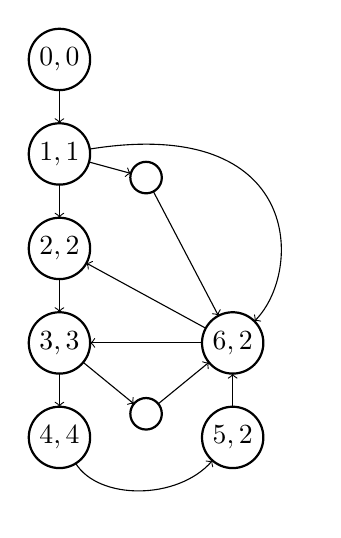
\begin{tikzpicture}
\tikzstyle{vertex}=[circle,thick, node distance = 12mm,
inner sep=2pt,outer sep=0pt,
draw=black,minimum height=4mm]
\node[vertex] at (0,0)	(0) { $0,0$ };
\node[vertex,below of =0,](1) {$1,1$} ;
\node[vertex,below of =1,](2) {$2,2$} ;
\node[vertex,below of =2,](3) {$3,3$} ;
\node[vertex,below of =3,](4) {$4,4$} ;
\node[vertex,right of =4,xshift=10mm](5) {$5,2$} ;
\node[right of =4,xshift=-5mm,yshift=-8mm](5c1) {};
\node[right of =4,xshift=5mm,yshift=-8mm](5c2) {};
\node[vertex,above of =5,](6) {$6,2$} ;
\node[vertex,right of =3,xshift=-1mm,yshift=-9mm](7) {$$} ;
\node[vertex,right of =2,xshift=-1mm,yshift=+9mm](8) {$$} ;

\node[right of =8,xshift=10mm,yshift=8mm](1c1) {};
\node[right of =8,xshift=10mm,yshift=-12mm](1c2) {};

\draw[->] (4) .. controls (5c1) and (5c2) ..  (5) ;
\draw[->] (1) .. controls (1c1) and (1c2) ..  (6) ;
\path[->] (0) edge (1) ;
\path[->] (1) edge (2) ;
\path[->] (1) edge (8) ;
\path[->] (8) edge (6) ;
\path[->] (2) edge (3) ;
\path[->] (3) edge (4) ;
\path[->] (5) edge (6) ;
\path[->] (3) edge (7) ;
\path[->] (7) edge (6) ;
\path[->] (6) edge (3) ;
\path[->] (6) edge (2) ;

\end{tikzpicture}
}
\end{column}
\begin{column}{1cm}
\begin{tabular}{|c|}
\hline
\\
\hline
\\
\hline
$6$\\
\hline
$5$\\
\hline
$4$\\
\hline
$3$\\
\hline
$2$\\
\hline
$1$\\
\hline
$0$\\
\hline
\end{tabular}\\
stack
\end{column}
\end{columns}
\end{frame}





% @@

\begin{frame}[fragile=singleslide]
\frametitle{Tarjan's Algorithm: More Processing of $4$}

\begin{columns}
\begin{column}{4cm}
{\tiny
\begin{itemize}
\item New lowlink and remains.
\end{itemize}

\begin{tabbing}
\ahdr
\INT \>\ID{dfnum}\>\>\>\>\>\\
								\\
\PROC \CALL{strong\_connect}($v$)				\\
\>\CALL{dfn}($v$) \ASGN \ID{dfnum}				\\
\>\CALL{lowlink}($v$) \ASGN \ID{dfnum}				\\ 
\>\CALL{visited}($v$) \ASGN true				\\
\>\CALL{push}($v$) 						\\
\>\ID{dfnum} \ASGN \ID{dfnum} $ + 1$				\\
								\\
\>\FOR each $w \in succ(v)$ \DO	\\
\>\>\IF (\NOT \CALL{visited}($w$)) \{				\\
\>\>\>\CALL{strong\_connect}($w$)				\\
\>\>\>\CALL{lowlink}($v$) \ASGN \CALL{min}(\CALL{lowlink}($v$), \CALL{lowlink}($w$))\\
\>\>\} \ELIF (\CALL{dfn}($w$) $ < $ \CALL{dfn}($v$) \AND $w$ is on stack)\\
\>\>\>\CALL{lowlink}($v$) \ASGN \CALL{min}(\CALL{lowlink}($v$), \CALL{dfn}($w$))\\
\\
\>\IF (\CALL{lowlink}($v$) $=$ \CALL{dfn}($v$)) 		\\
\>\>\ID{scc} \ASGN \EMPTY					\\
\>\>\DO								\\
\>\>\>$w$ \ASGN \CALL{pop}()					\\
\>\>\>add $w$ to \ID{scc}					\\
\>\>\WHILE ($w \neq v$)						\\
\>\>\CALL{process\_scc}(\ID{scc})				\\
\END
\end{tabbing}
}

\end{column}
\begin{column}{4cm}
{\tiny
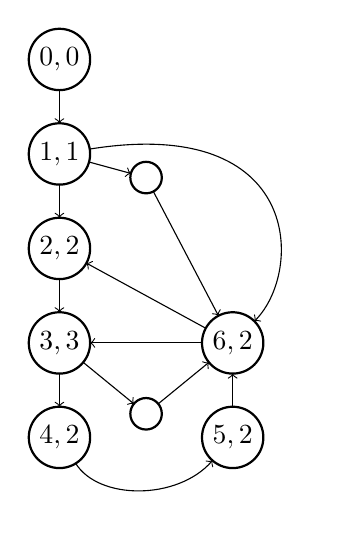
\begin{tikzpicture}
\tikzstyle{vertex}=[circle,thick, node distance = 12mm,
inner sep=2pt,outer sep=0pt,
draw=black,minimum height=4mm]
\node[vertex] at (0,0)	(0) { $0,0$ };
\node[vertex,below of =0,](1) {$1,1$} ;
\node[vertex,below of =1,](2) {$2,2$} ;
\node[vertex,below of =2,](3) {$3,3$} ;
\node[vertex,below of =3,](4) {$4,2$} ;
\node[vertex,right of =4,xshift=10mm](5) {$5,2$} ;
\node[right of =4,xshift=-5mm,yshift=-8mm](5c1) {};
\node[right of =4,xshift=5mm,yshift=-8mm](5c2) {};
\node[vertex,above of =5,](6) {$6,2$} ;
\node[vertex,right of =3,xshift=-1mm,yshift=-9mm](7) {$$} ;
\node[vertex,right of =2,xshift=-1mm,yshift=+9mm](8) {$$} ;

\node[right of =8,xshift=10mm,yshift=8mm](1c1) {};
\node[right of =8,xshift=10mm,yshift=-12mm](1c2) {};

\draw[->] (4) .. controls (5c1) and (5c2) ..  (5) ;
\draw[->] (1) .. controls (1c1) and (1c2) ..  (6) ;
\path[->] (0) edge (1) ;
\path[->] (1) edge (2) ;
\path[->] (1) edge (8) ;
\path[->] (8) edge (6) ;
\path[->] (2) edge (3) ;
\path[->] (3) edge (4) ;
\path[->] (5) edge (6) ;
\path[->] (3) edge (7) ;
\path[->] (7) edge (6) ;
\path[->] (6) edge (3) ;
\path[->] (6) edge (2) ;

\end{tikzpicture}
}
\end{column}
\begin{column}{1cm}
\begin{tabular}{|c|}
\hline
\\
\hline
\\
\hline
$6$\\
\hline
$5$\\
\hline
$4$\\
\hline
$3$\\
\hline
$2$\\
\hline
$1$\\
\hline
$0$\\
\hline
\end{tabular}\\
stack
\end{column}
\end{columns}
\end{frame}


% @@

\begin{frame}[fragile=singleslide]
\frametitle{Tarjan's Algorithm: More Processing of $3$}

\begin{columns}
\begin{column}{4cm}
{\tiny
\begin{itemize}
\item New lowlink. Next $7$.
\end{itemize}

\begin{tabbing}
\ahdr
\INT \>\ID{dfnum}\>\>\>\>\>\\
								\\
\PROC \CALL{strong\_connect}($v$)				\\
\>\CALL{dfn}($v$) \ASGN \ID{dfnum}				\\
\>\CALL{lowlink}($v$) \ASGN \ID{dfnum}				\\ 
\>\CALL{visited}($v$) \ASGN true				\\
\>\CALL{push}($v$) 						\\
\>\ID{dfnum} \ASGN \ID{dfnum} $ + 1$				\\
								\\
\>\FOR each $w \in succ(v)$ \DO	\\
\>\>\IF (\NOT \CALL{visited}($w$)) \{				\\
\>\>\>\CALL{strong\_connect}($w$)				\\
\>\>\>\CALL{lowlink}($v$) \ASGN \CALL{min}(\CALL{lowlink}($v$), \CALL{lowlink}($w$))\\
\>\>\} \ELIF (\CALL{dfn}($w$) $ < $ \CALL{dfn}($v$) \AND $w$ is on stack)\\
\>\>\>\CALL{lowlink}($v$) \ASGN \CALL{min}(\CALL{lowlink}($v$), \CALL{dfn}($w$))\\
\\
\>\IF (\CALL{lowlink}($v$) $=$ \CALL{dfn}($v$)) 		\\
\>\>\ID{scc} \ASGN \EMPTY					\\
\>\>\DO								\\
\>\>\>$w$ \ASGN \CALL{pop}()					\\
\>\>\>add $w$ to \ID{scc}					\\
\>\>\WHILE ($w \neq v$)						\\
\>\>\CALL{process\_scc}(\ID{scc})				\\
\END
\end{tabbing}
}

\end{column}
\begin{column}{4cm}
{\tiny
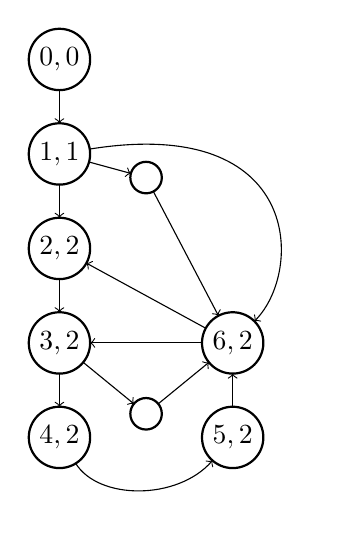
\begin{tikzpicture}
\tikzstyle{vertex}=[circle,thick, node distance = 12mm,
inner sep=2pt,outer sep=0pt,
draw=black,minimum height=4mm]
\node[vertex] at (0,0)	(0) { $0,0$ };
\node[vertex,below of =0,](1) {$1,1$} ;
\node[vertex,below of =1,](2) {$2,2$} ;
\node[vertex,below of =2,](3) {$3,2$} ;
\node[vertex,below of =3,](4) {$4,2$} ;
\node[vertex,right of =4,xshift=10mm](5) {$5,2$} ;
\node[right of =4,xshift=-5mm,yshift=-8mm](5c1) {};
\node[right of =4,xshift=5mm,yshift=-8mm](5c2) {};
\node[vertex,above of =5,](6) {$6,2$} ;
\node[vertex,right of =3,xshift=-1mm,yshift=-9mm](7) {$$} ;
\node[vertex,right of =2,xshift=-1mm,yshift=+9mm](8) {$$} ;

\node[right of =8,xshift=10mm,yshift=8mm](1c1) {};
\node[right of =8,xshift=10mm,yshift=-12mm](1c2) {};

\draw[->] (4) .. controls (5c1) and (5c2) ..  (5) ;
\draw[->] (1) .. controls (1c1) and (1c2) ..  (6) ;
\path[->] (0) edge (1) ;
\path[->] (1) edge (2) ;
\path[->] (1) edge (8) ;
\path[->] (8) edge (6) ;
\path[->] (2) edge (3) ;
\path[->] (3) edge (4) ;
\path[->] (5) edge (6) ;
\path[->] (3) edge (7) ;
\path[->] (7) edge (6) ;
\path[->] (6) edge (3) ;
\path[->] (6) edge (2) ;

\end{tikzpicture}
}
\end{column}
\begin{column}{1cm}
\begin{tabular}{|c|}
\hline
\\
\hline
\\
\hline
$6$\\
\hline
$5$\\
\hline
$4$\\
\hline
$3$\\
\hline
$2$\\
\hline
$1$\\
\hline
$0$\\
\hline
\end{tabular}\\
stack
\end{column}
\end{columns}
\end{frame}




% @@

\begin{frame}[fragile=singleslide]
\frametitle{Tarjan's Algorithm: Processing of $7$}

\begin{columns}
\begin{column}{4cm}
{\tiny
\begin{itemize}
\item Lowlink is set.
\end{itemize}

\begin{tabbing}
\ahdr
\INT \>\ID{dfnum}\>\>\>\>\>\\
								\\
\PROC \CALL{strong\_connect}($v$)				\\
\>\CALL{dfn}($v$) \ASGN \ID{dfnum}				\\
\>\CALL{lowlink}($v$) \ASGN \ID{dfnum}				\\ 
\>\CALL{visited}($v$) \ASGN true				\\
\>\CALL{push}($v$) 						\\
\>\ID{dfnum} \ASGN \ID{dfnum} $ + 1$				\\
								\\
\>\FOR each $w \in succ(v)$ \DO	\\
\>\>\IF (\NOT \CALL{visited}($w$)) \{				\\
\>\>\>\CALL{strong\_connect}($w$)				\\
\>\>\>\CALL{lowlink}($v$) \ASGN \CALL{min}(\CALL{lowlink}($v$), \CALL{lowlink}($w$))\\
\>\>\} \ELIF (\CALL{dfn}($w$) $ < $ \CALL{dfn}($v$) \AND $w$ is on stack)\\
\>\>\>\CALL{lowlink}($v$) \ASGN \CALL{min}(\CALL{lowlink}($v$), \CALL{dfn}($w$))\\
\\
\>\IF (\CALL{lowlink}($v$) $=$ \CALL{dfn}($v$)) 		\\
\>\>\ID{scc} \ASGN \EMPTY					\\
\>\>\DO								\\
\>\>\>$w$ \ASGN \CALL{pop}()					\\
\>\>\>add $w$ to \ID{scc}					\\
\>\>\WHILE ($w \neq v$)						\\
\>\>\CALL{process\_scc}(\ID{scc})				\\
\END
\end{tabbing}
}

\end{column}
\begin{column}{4cm}
{\tiny
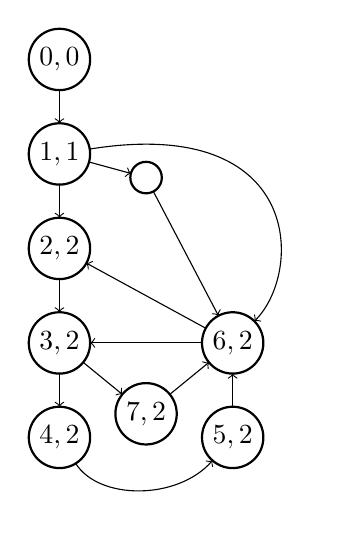
\begin{tikzpicture}
\tikzstyle{vertex}=[circle,thick, node distance = 12mm,
inner sep=2pt,outer sep=0pt,
draw=black,minimum height=4mm]
\node[vertex] at (0,0)	(0) { $0,0$ };
\node[vertex,below of =0,](1) {$1,1$} ;
\node[vertex,below of =1,](2) {$2,2$} ;
\node[vertex,below of =2,](3) {$3,2$} ;
\node[vertex,below of =3,](4) {$4,2$} ;
\node[vertex,right of =4,xshift=10mm](5) {$5,2$} ;
\node[right of =4,xshift=-5mm,yshift=-8mm](5c1) {};
\node[right of =4,xshift=5mm,yshift=-8mm](5c2) {};
\node[vertex,above of =5,](6) {$6,2$} ;
\node[vertex,right of =3,xshift=-1mm,yshift=-9mm](7) {$7,2$} ;
\node[vertex,right of =2,xshift=-1mm,yshift=+9mm](8) {$$} ;

\node[right of =8,xshift=10mm,yshift=8mm](1c1) {};
\node[right of =8,xshift=10mm,yshift=-12mm](1c2) {};

\draw[->] (4) .. controls (5c1) and (5c2) ..  (5) ;
\draw[->] (1) .. controls (1c1) and (1c2) ..  (6) ;
\path[->] (0) edge (1) ;
\path[->] (1) edge (2) ;
\path[->] (1) edge (8) ;
\path[->] (8) edge (6) ;
\path[->] (2) edge (3) ;
\path[->] (3) edge (4) ;
\path[->] (5) edge (6) ;
\path[->] (3) edge (7) ;
\path[->] (7) edge (6) ;
\path[->] (6) edge (3) ;
\path[->] (6) edge (2) ;

\end{tikzpicture}
}
\end{column}
\begin{column}{1cm}
\begin{tabular}{|c|}
\hline
\\
\hline
$7$\\
\hline
$6$\\
\hline
$5$\\
\hline
$4$\\
\hline
$3$\\
\hline
$2$\\
\hline
$1$\\
\hline
$0$\\
\hline
\end{tabular}\\
stack
\end{column}
\end{columns}
\end{frame}



% @@

\begin{frame}[fragile=singleslide]
\frametitle{Tarjan's Algorithm: More Processing of $2$}

\begin{columns}
\begin{column}{4cm}
{\tiny
\begin{itemize}
\item Remove SCC from stack
\end{itemize}

\begin{tabbing}
\ahdr
\INT \>\ID{dfnum}\>\>\>\>\>\\
								\\
\PROC \CALL{strong\_connect}($v$)				\\
\>\CALL{dfn}($v$) \ASGN \ID{dfnum}				\\
\>\CALL{lowlink}($v$) \ASGN \ID{dfnum}				\\ 
\>\CALL{visited}($v$) \ASGN true				\\
\>\CALL{push}($v$) 						\\
\>\ID{dfnum} \ASGN \ID{dfnum} $ + 1$				\\
								\\
\>\FOR each $w \in succ(v)$ \DO	\\
\>\>\IF (\NOT \CALL{visited}($w$)) \{				\\
\>\>\>\CALL{strong\_connect}($w$)				\\
\>\>\>\CALL{lowlink}($v$) \ASGN \CALL{min}(\CALL{lowlink}($v$), \CALL{lowlink}($w$))\\
\>\>\} \ELIF (\CALL{dfn}($w$) $ < $ \CALL{dfn}($v$) \AND $w$ is on stack)\\
\>\>\>\CALL{lowlink}($v$) \ASGN \CALL{min}(\CALL{lowlink}($v$), \CALL{dfn}($w$))\\
\\
\>\IF (\CALL{lowlink}($v$) $=$ \CALL{dfn}($v$)) 		\\
\>\>\ID{scc} \ASGN \EMPTY					\\
\>\>\DO								\\
\>\>\>$w$ \ASGN \CALL{pop}()					\\
\>\>\>add $w$ to \ID{scc}					\\
\>\>\WHILE ($w \neq v$)						\\
\>\>\CALL{process\_scc}(\ID{scc})				\\
\END
\end{tabbing}
}

\end{column}
\begin{column}{4cm}
{\tiny
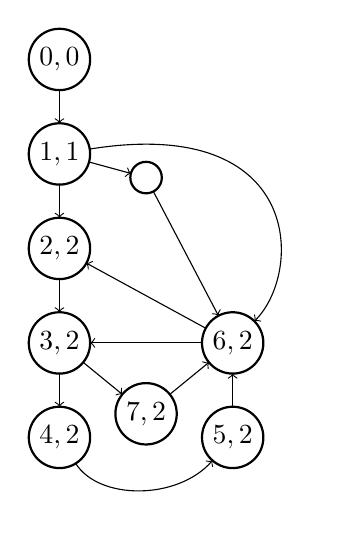
\begin{tikzpicture}
\tikzstyle{vertex}=[circle,thick, node distance = 12mm,
inner sep=2pt,outer sep=0pt,
draw=black,minimum height=4mm]
\node[vertex] at (0,0)	(0) { $0,0$ };
\node[vertex,below of =0,](1) {$1,1$} ;
\node[vertex,below of =1,](2) {$2,2$} ;
\node[vertex,below of =2,](3) {$3,2$} ;
\node[vertex,below of =3,](4) {$4,2$} ;
\node[vertex,right of =4,xshift=10mm](5) {$5,2$} ;
\node[right of =4,xshift=-5mm,yshift=-8mm](5c1) {};
\node[right of =4,xshift=5mm,yshift=-8mm](5c2) {};
\node[vertex,above of =5,](6) {$6,2$} ;
\node[vertex,right of =3,xshift=-1mm,yshift=-9mm](7) {$7,2$} ;
\node[vertex,right of =2,xshift=-1mm,yshift=+9mm](8) {$$} ;

\node[right of =8,xshift=10mm,yshift=8mm](1c1) {};
\node[right of =8,xshift=10mm,yshift=-12mm](1c2) {};

\draw[->] (4) .. controls (5c1) and (5c2) ..  (5) ;
\draw[->] (1) .. controls (1c1) and (1c2) ..  (6) ;
\path[->] (0) edge (1) ;
\path[->] (1) edge (2) ;
\path[->] (1) edge (8) ;
\path[->] (8) edge (6) ;
\path[->] (2) edge (3) ;
\path[->] (3) edge (4) ;
\path[->] (5) edge (6) ;
\path[->] (3) edge (7) ;
\path[->] (7) edge (6) ;
\path[->] (6) edge (3) ;
\path[->] (6) edge (2) ;

\end{tikzpicture}
}
\end{column}
\begin{column}{1cm}
\begin{tabular}{|c|}
\hline
\\
\hline
\\
\hline
\\
\hline
\\
\hline
\\
\hline
\\
\hline
\\
\hline
$1$\\
\hline
$0$\\
\hline
\end{tabular}\\
stack
\end{column}
\end{columns}
\end{frame}



% @@

\begin{frame}[fragile=singleslide]
\frametitle{Tarjan's Algorithm: Initial Processing of $8$}

\begin{columns}
\begin{column}{4cm}
{\tiny
\begin{itemize}
\item No path from $2$ to $8$.
\end{itemize}

\begin{tabbing}
\ahdr
\INT \>\ID{dfnum}\>\>\>\>\>\\
								\\
\PROC \CALL{strong\_connect}($v$)				\\
\>\CALL{dfn}($v$) \ASGN \ID{dfnum}				\\
\>\CALL{lowlink}($v$) \ASGN \ID{dfnum}				\\ 
\>\CALL{visited}($v$) \ASGN true				\\
\>\CALL{push}($v$) 						\\
\>\ID{dfnum} \ASGN \ID{dfnum} $ + 1$				\\
								\\
\>\FOR each $w \in succ(v)$ \DO	\\
\>\>\IF (\NOT \CALL{visited}($w$)) \{				\\
\>\>\>\CALL{strong\_connect}($w$)				\\
\>\>\>\CALL{lowlink}($v$) \ASGN \CALL{min}(\CALL{lowlink}($v$), \CALL{lowlink}($w$))\\
\>\>\} \ELIF (\CALL{dfn}($w$) $ < $ \CALL{dfn}($v$) \AND $w$ is on stack)\\
\>\>\>\CALL{lowlink}($v$) \ASGN \CALL{min}(\CALL{lowlink}($v$), \CALL{dfn}($w$))\\
\\
\>\IF (\CALL{lowlink}($v$) $=$ \CALL{dfn}($v$)) 		\\
\>\>\ID{scc} \ASGN \EMPTY					\\
\>\>\DO								\\
\>\>\>$w$ \ASGN \CALL{pop}()					\\
\>\>\>add $w$ to \ID{scc}					\\
\>\>\WHILE ($w \neq v$)						\\
\>\>\CALL{process\_scc}(\ID{scc})				\\
\END
\end{tabbing}
}

\end{column}
\begin{column}{4cm}
{\tiny
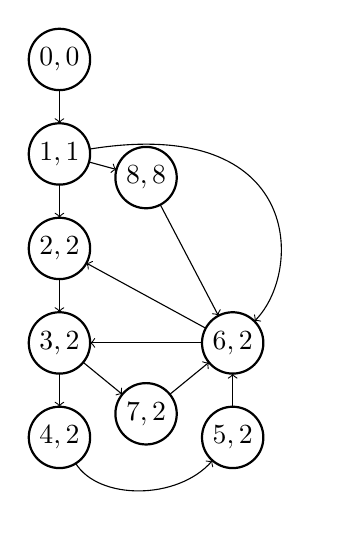
\begin{tikzpicture}
\tikzstyle{vertex}=[circle,thick, node distance = 12mm,
inner sep=2pt,outer sep=0pt,
draw=black,minimum height=4mm]
\node[vertex] at (0,0)	(0) { $0,0$ };
\node[vertex,below of =0,](1) {$1,1$} ;
\node[vertex,below of =1,](2) {$2,2$} ;
\node[vertex,below of =2,](3) {$3,2$} ;
\node[vertex,below of =3,](4) {$4,2$} ;
\node[vertex,right of =4,xshift=10mm](5) {$5,2$} ;
\node[right of =4,xshift=-5mm,yshift=-8mm](5c1) {};
\node[right of =4,xshift=5mm,yshift=-8mm](5c2) {};
\node[vertex,above of =5,](6) {$6,2$} ;
\node[vertex,right of =3,xshift=-1mm,yshift=-9mm](7) {$7,2$} ;
\node[vertex,right of =2,xshift=-1mm,yshift=+9mm](8) {$8,8$} ;

\node[right of =8,xshift=10mm,yshift=8mm](1c1) {};
\node[right of =8,xshift=10mm,yshift=-12mm](1c2) {};

\draw[->] (4) .. controls (5c1) and (5c2) ..  (5) ;
\draw[->] (1) .. controls (1c1) and (1c2) ..  (6) ;
\path[->] (0) edge (1) ;
\path[->] (1) edge (2) ;
\path[->] (1) edge (8) ;
\path[->] (8) edge (6) ;
\path[->] (2) edge (3) ;
\path[->] (3) edge (4) ;
\path[->] (5) edge (6) ;
\path[->] (3) edge (7) ;
\path[->] (7) edge (6) ;
\path[->] (6) edge (3) ;
\path[->] (6) edge (2) ;

\end{tikzpicture}
}
\end{column}
\begin{column}{1cm}
\begin{tabular}{|c|}
\hline
\\
\hline
\\
\hline
\\
\hline
\\
\hline
\\
\hline
\\
\hline
$8$\\
\hline
$1$\\
\hline
$0$\\
\hline
\end{tabular}\\
stack
\end{column}
\end{columns}
\end{frame}





% @@

\begin{frame}[fragile=singleslide]
\frametitle{Tarjan's Algorithm: More Processing of $8$}

\begin{columns}
\begin{column}{4cm}
{\tiny
\begin{itemize}
\item $8$ is its own SCC.
\end{itemize}

\begin{tabbing}
\ahdr
\INT \>\ID{dfnum}\>\>\>\>\>\\
								\\
\PROC \CALL{strong\_connect}($v$)				\\
\>\CALL{dfn}($v$) \ASGN \ID{dfnum}				\\
\>\CALL{lowlink}($v$) \ASGN \ID{dfnum}				\\ 
\>\CALL{visited}($v$) \ASGN true				\\
\>\CALL{push}($v$) 						\\
\>\ID{dfnum} \ASGN \ID{dfnum} $ + 1$				\\
								\\
\>\FOR each $w \in succ(v)$ \DO	\\
\>\>\IF (\NOT \CALL{visited}($w$)) \{				\\
\>\>\>\CALL{strong\_connect}($w$)				\\
\>\>\>\CALL{lowlink}($v$) \ASGN \CALL{min}(\CALL{lowlink}($v$), \CALL{lowlink}($w$))\\
\>\>\} \ELIF (\CALL{dfn}($w$) $ < $ \CALL{dfn}($v$) \AND $w$ is on stack)\\
\>\>\>\CALL{lowlink}($v$) \ASGN \CALL{min}(\CALL{lowlink}($v$), \CALL{dfn}($w$))\\
\\
\>\IF (\CALL{lowlink}($v$) $=$ \CALL{dfn}($v$)) 		\\
\>\>\ID{scc} \ASGN \EMPTY					\\
\>\>\DO								\\
\>\>\>$w$ \ASGN \CALL{pop}()					\\
\>\>\>add $w$ to \ID{scc}					\\
\>\>\WHILE ($w \neq v$)						\\
\>\>\CALL{process\_scc}(\ID{scc})				\\
\END
\end{tabbing}
}

\end{column}
\begin{column}{4cm}
{\tiny
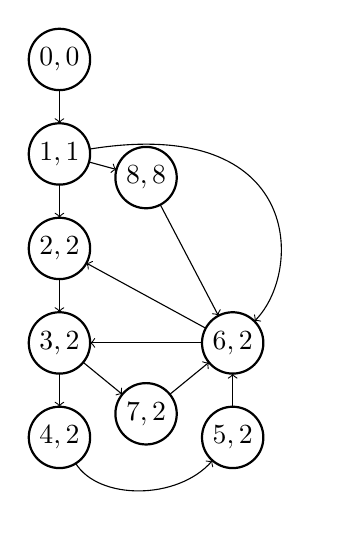
\begin{tikzpicture}
\tikzstyle{vertex}=[circle,thick, node distance = 12mm,
inner sep=2pt,outer sep=0pt,
draw=black,minimum height=4mm]
\node[vertex] at (0,0)	(0) { $0,0$ };
\node[vertex,below of =0,](1) {$1,1$} ;
\node[vertex,below of =1,](2) {$2,2$} ;
\node[vertex,below of =2,](3) {$3,2$} ;
\node[vertex,below of =3,](4) {$4,2$} ;
\node[vertex,right of =4,xshift=10mm](5) {$5,2$} ;
\node[right of =4,xshift=-5mm,yshift=-8mm](5c1) {};
\node[right of =4,xshift=5mm,yshift=-8mm](5c2) {};
\node[vertex,above of =5,](6) {$6,2$} ;
\node[vertex,right of =3,xshift=-1mm,yshift=-9mm](7) {$7,2$} ;
\node[vertex,right of =2,xshift=-1mm,yshift=+9mm](8) {$8,8$} ;

\node[right of =8,xshift=10mm,yshift=8mm](1c1) {};
\node[right of =8,xshift=10mm,yshift=-12mm](1c2) {};

\draw[->] (4) .. controls (5c1) and (5c2) ..  (5) ;
\draw[->] (1) .. controls (1c1) and (1c2) ..  (6) ;
\path[->] (0) edge (1) ;
\path[->] (1) edge (2) ;
\path[->] (1) edge (8) ;
\path[->] (8) edge (6) ;
\path[->] (2) edge (3) ;
\path[->] (3) edge (4) ;
\path[->] (5) edge (6) ;
\path[->] (3) edge (7) ;
\path[->] (7) edge (6) ;
\path[->] (6) edge (3) ;
\path[->] (6) edge (2) ;

\end{tikzpicture}
}
\end{column}
\begin{column}{1cm}
\begin{tabular}{|c|}
\hline
\\
\hline
\\
\hline
\\
\hline
\\
\hline
\\
\hline
\\
\hline
\\
\hline
$1$\\
\hline
$0$\\
\hline
\end{tabular}\\
stack
\end{column}
\end{columns}
\end{frame}




% @@

\begin{frame}[fragile=singleslide]
\frametitle{Tarjan's Algorithm: More Processing of $1$}

\begin{columns}
\begin{column}{4cm}
{\tiny
\begin{itemize}
\item $1$ is its own SCC.
\end{itemize}

\begin{tabbing}
\ahdr
\INT \>\ID{dfnum}\>\>\>\>\>\\
								\\
\PROC \CALL{strong\_connect}($v$)				\\
\>\CALL{dfn}($v$) \ASGN \ID{dfnum}				\\
\>\CALL{lowlink}($v$) \ASGN \ID{dfnum}				\\ 
\>\CALL{visited}($v$) \ASGN true				\\
\>\CALL{push}($v$) 						\\
\>\ID{dfnum} \ASGN \ID{dfnum} $ + 1$				\\
								\\
\>\FOR each $w \in succ(v)$ \DO	\\
\>\>\IF (\NOT \CALL{visited}($w$)) \{				\\
\>\>\>\CALL{strong\_connect}($w$)				\\
\>\>\>\CALL{lowlink}($v$) \ASGN \CALL{min}(\CALL{lowlink}($v$), \CALL{lowlink}($w$))\\
\>\>\} \ELIF (\CALL{dfn}($w$) $ < $ \CALL{dfn}($v$) \AND $w$ is on stack)\\
\>\>\>\CALL{lowlink}($v$) \ASGN \CALL{min}(\CALL{lowlink}($v$), \CALL{dfn}($w$))\\
\\
\>\IF (\CALL{lowlink}($v$) $=$ \CALL{dfn}($v$)) 		\\
\>\>\ID{scc} \ASGN \EMPTY					\\
\>\>\DO								\\
\>\>\>$w$ \ASGN \CALL{pop}()					\\
\>\>\>add $w$ to \ID{scc}					\\
\>\>\WHILE ($w \neq v$)						\\
\>\>\CALL{process\_scc}(\ID{scc})				\\
\END
\end{tabbing}
}

\end{column}
\begin{column}{4cm}
{\tiny
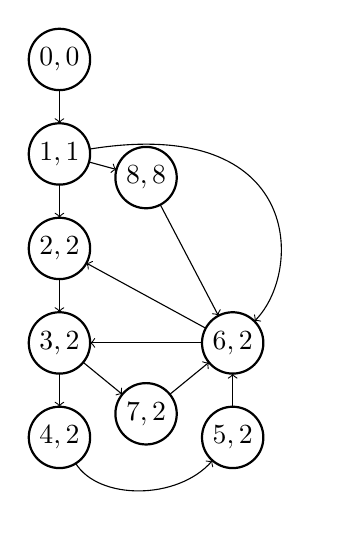
\begin{tikzpicture}
\tikzstyle{vertex}=[circle,thick, node distance = 12mm,
inner sep=2pt,outer sep=0pt,
draw=black,minimum height=4mm]
\node[vertex] at (0,0)	(0) { $0,0$ };
\node[vertex,below of =0,](1) {$1,1$} ;
\node[vertex,below of =1,](2) {$2,2$} ;
\node[vertex,below of =2,](3) {$3,2$} ;
\node[vertex,below of =3,](4) {$4,2$} ;
\node[vertex,right of =4,xshift=10mm](5) {$5,2$} ;
\node[right of =4,xshift=-5mm,yshift=-8mm](5c1) {};
\node[right of =4,xshift=5mm,yshift=-8mm](5c2) {};
\node[vertex,above of =5,](6) {$6,2$} ;
\node[vertex,right of =3,xshift=-1mm,yshift=-9mm](7) {$7,2$} ;
\node[vertex,right of =2,xshift=-1mm,yshift=+9mm](8) {$8,8$} ;

\node[right of =8,xshift=10mm,yshift=8mm](1c1) {};
\node[right of =8,xshift=10mm,yshift=-12mm](1c2) {};

\draw[->] (4) .. controls (5c1) and (5c2) ..  (5) ;
\draw[->] (1) .. controls (1c1) and (1c2) ..  (6) ;
\path[->] (0) edge (1) ;
\path[->] (1) edge (2) ;
\path[->] (1) edge (8) ;
\path[->] (8) edge (6) ;
\path[->] (2) edge (3) ;
\path[->] (3) edge (4) ;
\path[->] (5) edge (6) ;
\path[->] (3) edge (7) ;
\path[->] (7) edge (6) ;
\path[->] (6) edge (3) ;
\path[->] (6) edge (2) ;

\end{tikzpicture}
}
\end{column}
\begin{column}{1cm}
\begin{tabular}{|c|}
\hline
\\
\hline
\\
\hline
\\
\hline
\\
\hline
\\
\hline
\\
\hline
\\
\hline
\\
\hline
$0$\\
\hline
\end{tabular}\\
stack
\end{column}
\end{columns}
\end{frame}





% @@

\begin{frame}[fragile=singleslide]
\frametitle{Tarjan's Algorithm: More Processing of $0$}

\begin{columns}
\begin{column}{4cm}
{\tiny
\begin{itemize}
\item $0$ is its own SCC.
\end{itemize}

\begin{tabbing}
\ahdr
\INT \>\ID{dfnum}\>\>\>\>\>\\
								\\
\PROC \CALL{strong\_connect}($v$)				\\
\>\CALL{dfn}($v$) \ASGN \ID{dfnum}				\\
\>\CALL{lowlink}($v$) \ASGN \ID{dfnum}				\\ 
\>\CALL{visited}($v$) \ASGN true				\\
\>\CALL{push}($v$) 						\\
\>\ID{dfnum} \ASGN \ID{dfnum} $ + 1$				\\
								\\
\>\FOR each $w \in succ(v)$ \DO	\\
\>\>\IF (\NOT \CALL{visited}($w$)) \{				\\
\>\>\>\CALL{strong\_connect}($w$)				\\
\>\>\>\CALL{lowlink}($v$) \ASGN \CALL{min}(\CALL{lowlink}($v$), \CALL{lowlink}($w$))\\
\>\>\} \ELIF (\CALL{dfn}($w$) $ < $ \CALL{dfn}($v$) \AND $w$ is on stack)\\
\>\>\>\CALL{lowlink}($v$) \ASGN \CALL{min}(\CALL{lowlink}($v$), \CALL{dfn}($w$))\\
\\
\>\IF (\CALL{lowlink}($v$) $=$ \CALL{dfn}($v$)) 		\\
\>\>\ID{scc} \ASGN \EMPTY					\\
\>\>\DO								\\
\>\>\>$w$ \ASGN \CALL{pop}()					\\
\>\>\>add $w$ to \ID{scc}					\\
\>\>\WHILE ($w \neq v$)						\\
\>\>\CALL{process\_scc}(\ID{scc})				\\
\END
\end{tabbing}
}

\end{column}
\begin{column}{4cm}
{\tiny
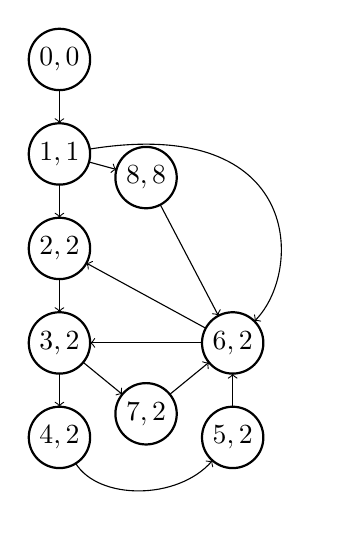
\begin{tikzpicture}
\tikzstyle{vertex}=[circle,thick, node distance = 12mm,
inner sep=2pt,outer sep=0pt,
draw=black,minimum height=4mm]
\node[vertex] at (0,0)	(0) { $0,0$ };
\node[vertex,below of =0,](1) {$1,1$} ;
\node[vertex,below of =1,](2) {$2,2$} ;
\node[vertex,below of =2,](3) {$3,2$} ;
\node[vertex,below of =3,](4) {$4,2$} ;
\node[vertex,right of =4,xshift=10mm](5) {$5,2$} ;
\node[right of =4,xshift=-5mm,yshift=-8mm](5c1) {};
\node[right of =4,xshift=5mm,yshift=-8mm](5c2) {};
\node[vertex,above of =5,](6) {$6,2$} ;
\node[vertex,right of =3,xshift=-1mm,yshift=-9mm](7) {$7,2$} ;
\node[vertex,right of =2,xshift=-1mm,yshift=+9mm](8) {$8,8$} ;

\node[right of =8,xshift=10mm,yshift=8mm](1c1) {};
\node[right of =8,xshift=10mm,yshift=-12mm](1c2) {};

\draw[->] (4) .. controls (5c1) and (5c2) ..  (5) ;
\draw[->] (1) .. controls (1c1) and (1c2) ..  (6) ;
\path[->] (0) edge (1) ;
\path[->] (1) edge (2) ;
\path[->] (1) edge (8) ;
\path[->] (8) edge (6) ;
\path[->] (2) edge (3) ;
\path[->] (3) edge (4) ;
\path[->] (5) edge (6) ;
\path[->] (3) edge (7) ;
\path[->] (7) edge (6) ;
\path[->] (6) edge (3) ;
\path[->] (6) edge (2) ;

\end{tikzpicture}
}
\end{column}
\begin{column}{1cm}
\begin{tabular}{|c|}
\hline
\\
\hline
\\
\hline
\\
\hline
\\
\hline
\\
\hline
\\
\hline
\\
\hline
\\
\hline
\\
\hline
\end{tabular}\\
stack
\end{column}
\end{columns}
\end{frame}



% @@

\begin{frame}[fragile=singleslide]
\frametitle{Tarjan's Algorithm: Remarks}

\begin{itemize}
\item Consider the edge $(v,w$).
\item When $w$ is not yet visited we must visit it by calling $strong\_connect(w)$.
\item If $w$ has been visited, we have two main cases: 
\begin{enumerate}
\item $w$ is not on the stack, because it has already found its SCC.
\item $w$ is on the stack, because it's waiting for being popped.
\begin{itemize}
\item If $dfn(w) < dfn(v)$ then $v$ must set its lowlink so it does not
think it is its own SCC.
\item If $dfn(w) \ge dfn(v)$ then no more information for $v$ is available. There is another path from $v$ to $w$ due to which they will belong to the same SCC.
\end{itemize}
\end{enumerate}
\end{itemize}
\end{frame}

\begin{frame}
\frametitle{Lab 2: Breadth-first search}
\begin{itemize}
\item Lab 2 is called Word Ladders
\item Two input files are to be read by the program --- not standard input as in Lab 1
\item The first file is a list of five character words
\item The second file contains two words per line
\item You should create a directed graph from the first file
\item Each word is a node, and there is an edge from $v$ to $w$ if each of the last 
four characters of $v$ appear in $w$.
\item All four last characters in $v$ must appear with repetition in $w$
\item T\underline{HERE} should have an edge to ETHER but not to RETCH (since one E is missing).
\end{itemize}
\end{frame}

\end{document}

\begin{frame}
\frametitle{Lab 2}
\begin{itemize}
\item Your program should then read the second file with word pairs $v$ and $w$
\item For each word pair, it should search the graph for a path from $v$ to $w$
\item The shortest distance should be printed on {\tt System.out} or -1 if no path from $v$ to $w$ exists
\item Your BFS should have time complexity $O(m+n)$ for $m$ edges and $n$ nodes.
\end{itemize}
\end{frame}

\begin{frame}[fragile=singleslide]
\frametitle{XXX}
\begin{itemize}
\item XXX
\end{itemize}
\end{frame}
